% !TEX program = xelatex
% 編譯方式： xelatex walk_導讀.tex   （在 notes/ 裡執行，跑兩次以產生目錄與交互參照）
% 內文在 ch1/part1.tex；圖與表由 ch1/make_figs.py 產生（ch1/figs.tex，含數字檢查）。先 python ch1/make_figs.py 再編譯。
\documentclass[11pt,a4paper]{article}

\usepackage[margin=2.2cm]{geometry}
\usepackage{amsmath,amssymb,mathtools}
\usepackage{xeCJK}
\setCJKmainfont[BoldFont={Microsoft JhengHei Bold},ItalicFont={DFKai-SB}]{Microsoft JhengHei}
\setCJKsansfont[BoldFont={Microsoft JhengHei Bold}]{Microsoft JhengHei}
\setCJKmonofont{Microsoft JhengHei}
\linespread{1.28}
\setlength{\parskip}{0.45em}
\setlength{\parindent}{0pt}

\usepackage{xcolor}
\usepackage{tikz}
\usetikzlibrary{calc,arrows.meta,positioning,decorations.markings}
\usepackage[most]{tcolorbox}
\usepackage{booktabs}
\usepackage{enumitem}
\setlist{itemsep=0.15em,topsep=0.3em}
\usepackage{float}
\usepackage{caption}
\captionsetup{font=small,labelfont=bf,labelsep=quad}
\renewcommand{\figurename}{圖}
\renewcommand{\tablename}{表}
\renewcommand{\contentsname}{目錄}
\usepackage[colorlinks=true,linkcolor=blue!50!black,urlcolor=blue!50!black]{hyperref}

% ---------- 顏色（與 manim 動畫 W101--W112 一致） ----------
\definecolor{cHead}{HTML}{D9A21B}      % 正面／向右（動畫：金）
\definecolor{cTail}{HTML}{4F7FA8}      % 反面／向左（動畫：藍灰）
\colorlet{cWalk}{orange!85!black}      % 主例路線（動畫：黃）
\colorlet{cBar}{blue!60!black}         % 精確值的長條
\colorlet{cGauss}{orange!90!black}     % 高斯近似
\colorlet{cExact}{green!45!black}      % 精確值、更正
\colorlet{cWrong}{red!80!black}        % 書上的筆誤

% ---------- 盒子 ----------
\newtcolorbox{keybox}[1][]{enhanced,breakable,colback=blue!4,colframe=blue!45!black,
  boxrule=0.7pt,arc=2pt,left=8pt,right=8pt,top=5pt,bottom=5pt,fonttitle=\bfseries,title={#1}}
\newtcolorbox{thmbox}[1][]{enhanced,breakable,colback=orange!7,colframe=orange!75!black,
  boxrule=0.8pt,arc=2pt,left=8pt,right=8pt,top=5pt,bottom=5pt,fonttitle=\bfseries,title={#1}}
\newtcolorbox{notebox}[1][]{enhanced,breakable,colback=gray!7,colframe=gray!60,
  boxrule=0.5pt,arc=2pt,left=8pt,right=8pt,top=5pt,bottom=5pt,fonttitle=\bfseries,title={#1}}
\newtcolorbox{errbox}[1][]{enhanced,breakable,colback=red!3,colframe=cWrong,
  boxrule=0.6pt,arc=2pt,left=8pt,right=8pt,top=4pt,bottom=4pt,fonttitle=\bfseries,title={書上筆誤　#1}}

\newcommand{\bk}[1]{{\small\color{gray!70!black}〔書 #1〕}}           % 書上的頁碼
\newcommand{\anim}[1]{{\small\color{cBar}〔動畫 #1〕}}                % 對應的 manim 動畫
\newcommand{\coinH}{\tikz[baseline=-0.65ex]\node[circle,fill=cHead!75,draw=cHead!60!black,inner sep=0.6pt,font=\scriptsize]{正};}
\newcommand{\coinT}{\tikz[baseline=-0.65ex]\node[circle,fill=cTail!45,draw=cTail!80!black,inner sep=0.6pt,font=\scriptsize]{反};}
\newcommand{\avg}[1]{\overline{#1}}

\begin{document}

\begin{center}
{\Large\bfseries 隨機漫步導讀}\\[4pt]
J.~Rudnick、G.~Gaspari《Elements of the Random Walk》第 1 章（配合 manim 動畫 W101--W112）\\[8pt]
{\small 原文：Joseph Rudnick and George Gaspari, \emph{Elements of the Random Walk: An Introduction for Advanced
Students and Researchers}, Cambridge University Press, 2004.}
\end{center}

\begin{keybox}[全書地圖（目前完成：第 1 章）]
\small
\begin{tabular}{@{}rp{0.93\linewidth}@{}}
1 & 技巧入門：一維最簡單的漫步——數路線、動差、Stirling 與高斯、擴散方程、生成函數、鞍點法（序曲）\\
2 & 生成函數 I：生成函數到底是什麼、格子上的漫步、長路線的漸近行為、普適性、連續極限與擴散\\
3 & 生成函數 II：回不回得了家（Pólya 的常返性）、維度的角色、走過幾個格點\\
4 & 邊界條件、穩定態與靜電類比：吸收牆、限制在區間或球裡、Fick 定律、電容的類比\\
5 & 漫步的變化形：有偏向的漫步、有慣性（persistent）的漫步、連續時間漫步\\
6 & 漫步的形狀：迴轉半徑張量、非球度、高維的 $1/d$ 展開\\
7 & 路徑積分與自迴避：把漫步寫成路徑積分、微擾展開、平均場、Flory 論證\\
8 & 標度入門：普適性、非高斯行為、維度與 Flory 指數\\
9 & 標度與臨界現象：$O(n)$ 模型、Ginzburg--Landau--Wilson 有效 Hamiltonian、自迴避漫步＝$n\to0$ 的磁鐵\\
10 & $O(n)$ 模型的平均場與自旋波；關聯洞\\
11 & 標度、碎形與重整化群：實空間方法、遞迴關係、固定點與臨界指數\\
12 & 重整化群（續）：動量殼方法、圖解法、兩點關聯函數
\end{tabular}

作者在前言說：前五章講「沒有記憶」的漫步，但刻意用生成函數的語言來講；第 7--12 章用同一套語言處理「不能走回頭路」的自迴避漫步，
並把它對應到磁性系統的臨界現象。所以第 1 章雖然簡單，每一個技巧後面都會再用到。
\end{keybox}

\begin{keybox}[第 1 章一頁看懂]
一個人每次擲硬幣：正面向右走一步、反面向左走一步（步長 $l$）。走了 $N$ 步之後——
\begin{enumerate}[nosep]
\item \textbf{停在哪裡？} 終點 $d$ 的走法數是二項式係數 $C(N,d)=\binom{N}{(N+d/l)/2}$，機率 $P(N,d)=C(N,d)/2^N$。
\item \textbf{平均離家多遠？} 平均位置 $0$，但均方位移 $\avg{x^2}=Nl^2$：距離只長成 $\sqrt N$。所有動差都能用生成函數「微分一下」算出。
\item \textbf{$N$ 很大時長什麼樣？} 用 Stirling 公式 $N!\approx\sqrt{2\pi N}\,N^Ne^{-N}$，二項分布變成高斯分布（中央極限定理）。
\item \textbf{換個角度：} 走法數滿足遞迴 $C(N)=C(N-1,\text{左鄰})+C(N-1,\text{右鄰})$（Pascal 三角形）；格子變細就是擴散方程
      $\partial P/\partial N=\frac{l^2}{2}\partial^2P/\partial y^2$。
\item \textbf{全書的主角：生成函數。} $C(N,d)$ 是 $(2\cos ql)^N$ 的傅立葉係數；再對 $N$ 加總得 $g(z,q)=1/(1-z\cdot2\cos ql)$。
      係數用 Cauchy 積分取出，$N$ 很大時用鞍點法（最陡下降法）估計。
\end{enumerate}
\end{keybox}

\setcounter{tocdepth}{2}
\begingroup
\setlength{\parskip}{0pt}
\tableofcontents
\endgroup

\begin{center}
\small
\begin{tabular}{@{}lll@{\qquad}lll@{}}
\toprule
節 & 內容 & 動畫 & 節 & 內容 & 動畫\\
\midrule
1.1 & 擲硬幣走路、數路線 & W101--W102 & 1.4 & 遞迴與擴散方程 & W108--W109\\
1.2 & 平均、均方、動差 & W103--W105 & 1.5 & 傅立葉與生成函數 & W110--W111\\
1.3 & Stirling 公式與高斯 & W106--W107 & 1.6 & 最陡下降法 & W112\\
\bottomrule
\end{tabular}
\end{center}

\noindent 以〔書 p.~5〕標示書上的頁碼，式號 (1.6) 等與書上相同。內文寫到的每一個數字都由程式（\texttt{codes/utils/walk1d.py}）重算，
圖表由 \texttt{ch1/make\_figs.py} 產生並先做數字檢查（路徑相對於 \texttt{C:\textbackslash mypython\textbackslash manim\textbackslash projects\textbackslash walk017}）。
書上有十幾處筆誤，在文中用紅框標出，總表在 1.7 節；逐式校對見 \texttt{ref/md/ch01\_formulas.md}。連續播放：\texttt{Ch1Demo}（W101--W112）。

% figs.tex —— 由 ch1/make_figs.py 產生，請勿手動修改。
% 重新產生：python ch1/make_figs.py（第 1 章，動畫 W101–W112）

\newcommand{\FigMainWalk}{%
\begin{tikzpicture}[x=0.82cm,y=0.42cm,>=Stealth]
\draw[gray!25] (0,-3) grid (10,3);
\draw[->] (0,0) -- (10.7,0) node[right]{\small 步數 $k$};
\draw[->] (0,-3.3) -- (0,3.9) node[above]{\small 位置 $x$};
\node[below,font=\scriptsize] at (2,0) {$2$};
\node[below,font=\scriptsize] at (4,0) {$4$};
\node[below,font=\scriptsize] at (6,0) {$6$};
\node[below,font=\scriptsize] at (8,0) {$8$};
\node[below,font=\scriptsize] at (10,0) {$10$};
\node[left,font=\scriptsize] at (0,-2) {$-2$};
\node[left,font=\scriptsize] at (0,2) {$2$};
\node at (0.5,3.45) {\coinH};
\node at (1.5,3.45) {\coinT};
\node at (2.5,3.45) {\coinH};
\node at (3.5,3.45) {\coinH};
\node at (4.5,3.45) {\coinT};
\node at (5.5,3.45) {\coinH};
\node at (6.5,3.45) {\coinT};
\node at (7.5,3.45) {\coinT};
\node at (8.5,3.45) {\coinH};
\node at (9.5,3.45) {\coinH};
\draw[cWalk,very thick] (0,0) -- (1,1) -- (2,0) -- (3,1) -- (4,2) -- (5,1) -- (6,2) -- (7,1) -- (8,0) -- (9,1) -- (10,2);
\fill[cWalk] (0,0) circle (2.2pt);
\fill[cWalk] (1,1) circle (2.2pt);
\fill[cWalk] (2,0) circle (2.2pt);
\fill[cWalk] (3,1) circle (2.2pt);
\fill[cWalk] (4,2) circle (2.2pt);
\fill[cWalk] (5,1) circle (2.2pt);
\fill[cWalk] (6,2) circle (2.2pt);
\fill[cWalk] (7,1) circle (2.2pt);
\fill[cWalk] (8,0) circle (2.2pt);
\fill[cWalk] (9,1) circle (2.2pt);
\fill[cWalk] (10,2) circle (2.2pt);
\node[right,font=\small] at (10,2) {$d=2$};
\end{tikzpicture}
}

\newcommand{\TabThreeCoins}{%
\begin{tabular}{cccc}
\toprule
正面數 $n$ & 序列 & 個數 $\binom3n$ & 終點 $d=2n-3$\\
\midrule
$3$ & \coinH\coinH\coinH & $1$ & $3$\\
$2$ & \coinH\coinH\coinT\quad \coinH\coinT\coinH\quad \coinT\coinH\coinH & $3$ & $1$\\
$1$ & \coinH\coinT\coinT\quad \coinT\coinH\coinT\quad \coinT\coinT\coinH & $3$ & $-1$\\
$0$ & \coinT\coinT\coinT & $1$ & $-3$\\
\bottomrule
\end{tabular}
}

\newcommand{\TabTenDist}{%
\begin{tabular}{lcccccc}
\toprule
終點 $d$ & $0$ & $2$ & $4$ & $6$ & $8$ & $10$\\
\midrule
走法數 $C(10,d)$ & $252$ & $210$ & $120$ & $45$ & $10$ & $1$\\
機率 $P(10,d)=C/1024$ & $0.2461$ & $0.2051$ & $0.1172$ & $0.0439$ & $0.0098$ & $0.0010$\\
高斯近似 $\frac{2}{\sqrt{20\pi}}e^{-d^2/20}$ & $0.2523$ & $0.2066$ & $0.1134$ & $0.0417$ & $0.0103$ & $0.0017$\\
\bottomrule
\end{tabular}
}

\newcommand{\FigDeltaGrid}{%
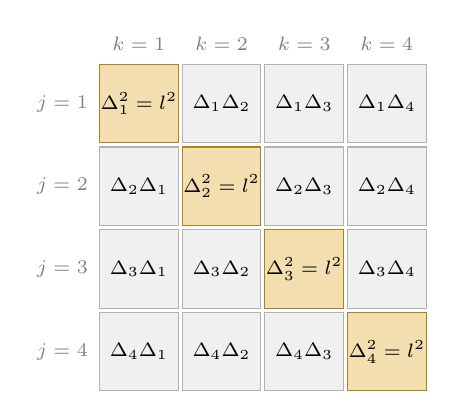
\begin{tikzpicture}[x=1.05cm,y=1.05cm]
\filldraw[fill=cHead!35,draw=cHead!80!black] (0,0) rectangle ++(0.95,0.95);
\node[font=\scriptsize] at (0.475,0.475) {$\Delta_1^2=l^2$};
\filldraw[fill=gray!12,draw=gray!60] (1,0) rectangle ++(0.95,0.95);
\node[font=\scriptsize] at (1.475,0.475) {$\Delta_1\Delta_2$};
\filldraw[fill=gray!12,draw=gray!60] (2,0) rectangle ++(0.95,0.95);
\node[font=\scriptsize] at (2.475,0.475) {$\Delta_1\Delta_3$};
\filldraw[fill=gray!12,draw=gray!60] (3,0) rectangle ++(0.95,0.95);
\node[font=\scriptsize] at (3.475,0.475) {$\Delta_1\Delta_4$};
\filldraw[fill=gray!12,draw=gray!60] (0,-1) rectangle ++(0.95,0.95);
\node[font=\scriptsize] at (0.475,-0.525) {$\Delta_2\Delta_1$};
\filldraw[fill=cHead!35,draw=cHead!80!black] (1,-1) rectangle ++(0.95,0.95);
\node[font=\scriptsize] at (1.475,-0.525) {$\Delta_2^2=l^2$};
\filldraw[fill=gray!12,draw=gray!60] (2,-1) rectangle ++(0.95,0.95);
\node[font=\scriptsize] at (2.475,-0.525) {$\Delta_2\Delta_3$};
\filldraw[fill=gray!12,draw=gray!60] (3,-1) rectangle ++(0.95,0.95);
\node[font=\scriptsize] at (3.475,-0.525) {$\Delta_2\Delta_4$};
\filldraw[fill=gray!12,draw=gray!60] (0,-2) rectangle ++(0.95,0.95);
\node[font=\scriptsize] at (0.475,-1.525) {$\Delta_3\Delta_1$};
\filldraw[fill=gray!12,draw=gray!60] (1,-2) rectangle ++(0.95,0.95);
\node[font=\scriptsize] at (1.475,-1.525) {$\Delta_3\Delta_2$};
\filldraw[fill=cHead!35,draw=cHead!80!black] (2,-2) rectangle ++(0.95,0.95);
\node[font=\scriptsize] at (2.475,-1.525) {$\Delta_3^2=l^2$};
\filldraw[fill=gray!12,draw=gray!60] (3,-2) rectangle ++(0.95,0.95);
\node[font=\scriptsize] at (3.475,-1.525) {$\Delta_3\Delta_4$};
\filldraw[fill=gray!12,draw=gray!60] (0,-3) rectangle ++(0.95,0.95);
\node[font=\scriptsize] at (0.475,-2.525) {$\Delta_4\Delta_1$};
\filldraw[fill=gray!12,draw=gray!60] (1,-3) rectangle ++(0.95,0.95);
\node[font=\scriptsize] at (1.475,-2.525) {$\Delta_4\Delta_2$};
\filldraw[fill=gray!12,draw=gray!60] (2,-3) rectangle ++(0.95,0.95);
\node[font=\scriptsize] at (2.475,-2.525) {$\Delta_4\Delta_3$};
\filldraw[fill=cHead!35,draw=cHead!80!black] (3,-3) rectangle ++(0.95,0.95);
\node[font=\scriptsize] at (3.475,-2.525) {$\Delta_4^2=l^2$};
\node[font=\scriptsize,gray] at (0.475,1.2) {$k=1$};
\node[font=\scriptsize,gray] at (-0.45,0.475) {$j=1$};
\node[font=\scriptsize,gray] at (1.475,1.2) {$k=2$};
\node[font=\scriptsize,gray] at (-0.45,-0.525) {$j=2$};
\node[font=\scriptsize,gray] at (2.475,1.2) {$k=3$};
\node[font=\scriptsize,gray] at (-0.45,-1.525) {$j=3$};
\node[font=\scriptsize,gray] at (3.475,1.2) {$k=4$};
\node[font=\scriptsize,gray] at (-0.45,-2.525) {$j=4$};
\end{tikzpicture}
}

\newcommand{\TabMoments}{%
\begin{tabular}{lcccccc}
\toprule
$N$ & $1$ & $2$ & $3$ & $4$ & $5$ & $6$\\
\midrule
$\overline{x^2}=N$ & $1$ & $2$ & $3$ & $4$ & $5$ & $6$\\
$\overline{x^4}=3N^2-2N$ & $1$ & $8$ & $21$ & $40$ & $65$ & $96$\\
$\overline{x^6}=15N^3-30N^2+16N$ & $1$ & $32$ & $183$ & $544$ & $1205$ & $2256$\\
$\overline{x^4}/(\overline{x^2})^2=3-2/N$ & $1$ & $2$ & $\tfrac{7}{3}$ & $\tfrac{5}{2}$ & $\tfrac{13}{5}$ & $\tfrac{8}{3}$\\
\bottomrule
\end{tabular}
}

\newcommand{\FigKurtosis}{%
\begin{tikzpicture}[x=0.62cm,y=1.1cm,>=Stealth]
\draw[->] (0,0) -- (10.8,0) node[right]{\small $N$};
\draw[->] (0,0) -- (0,3.5);
\draw[cGauss,dashed,thick] (0,3) -- (10.5,3) node[right,font=\small]{$3$（高斯）};
\fill[cBar] (1,1.0000) circle (2.4pt);
\node[below,font=\scriptsize] at (1,0) {$1$};
\fill[cBar] (2,2.0000) circle (2.4pt);
\node[below,font=\scriptsize] at (2,0) {$2$};
\fill[cBar] (3,2.3333) circle (2.4pt);
\node[below,font=\scriptsize] at (3,0) {$3$};
\fill[cBar] (4,2.5000) circle (2.4pt);
\node[below,font=\scriptsize] at (4,0) {$4$};
\fill[cBar] (5,2.6000) circle (2.4pt);
\node[below,font=\scriptsize] at (5,0) {$5$};
\fill[cBar] (6,2.6667) circle (2.4pt);
\node[below,font=\scriptsize] at (6,0) {$6$};
\fill[cBar] (7,2.7143) circle (2.4pt);
\node[below,font=\scriptsize] at (7,0) {$7$};
\fill[cBar] (8,2.7500) circle (2.4pt);
\node[below,font=\scriptsize] at (8,0) {$8$};
\fill[cBar] (9,2.7778) circle (2.4pt);
\node[below,font=\scriptsize] at (9,0) {$9$};
\fill[cBar] (10,2.8000) circle (2.4pt);
\node[below,font=\scriptsize] at (10,0) {$10$};
\draw (-0.08,1) -- (0.08,1) node[left=2pt,font=\scriptsize] {$1$};
\draw (-0.08,2) -- (0.08,2) node[left=2pt,font=\scriptsize] {$2$};
\end{tikzpicture}
}

\newcommand{\FigGamma}{%
\begin{tikzpicture}[x=0.3cm,y=0.75cm,>=Stealth]
\draw[->] (0,0) -- (31.5,0) node[right]{\small $w$};
\draw[->] (0,0) -- (0,5.3);
\draw (5,0.06) -- (5,-0.06) node[below,font=\scriptsize]{$5$};
\draw (10,0.06) -- (10,-0.06) node[below,font=\scriptsize]{$10$};
\draw (15,0.06) -- (15,-0.06) node[below,font=\scriptsize]{$15$};
\draw (20,0.06) -- (20,-0.06) node[below,font=\scriptsize]{$20$};
\draw (25,0.06) -- (25,-0.06) node[below,font=\scriptsize]{$25$};
\draw (30,0.06) -- (30,-0.06) node[below,font=\scriptsize]{$30$};
\draw (0.3,1) -- (-0.3,1) node[left,font=\scriptsize]{$1\times10^5$};
\draw (0.3,2) -- (-0.3,2) node[left,font=\scriptsize]{$2\times10^5$};
\draw (0.3,3) -- (-0.3,3) node[left,font=\scriptsize]{$3\times10^5$};
\draw (0.3,4) -- (-0.3,4) node[left,font=\scriptsize]{$4\times10^5$};
\draw[cBar,thick] plot coordinates {(0.00,0.0000) (0.25,0.0000) (0.50,0.0000) (0.75,0.0000) (1.00,0.0000) (1.25,0.0000) (1.50,0.0001) (1.75,0.0005) (2.00,0.0014) (2.25,0.0035) (2.50,0.0078) (2.75,0.0158) (3.00,0.0294) (3.25,0.0510) (3.50,0.0833) (3.75,0.1293) (4.00,0.1921) (4.25,0.2742) (4.50,0.3783) (4.75,0.5059) (5.00,0.6580) (5.25,0.8347) (5.50,1.0352) (5.75,1.2574) (6.00,1.4988) (6.25,1.7557) (6.50,2.0240) (6.75,2.2991) (7.00,2.5758) (7.25,2.8493) (7.50,3.1146) (7.75,3.3669) (8.00,3.6020) (8.25,3.8160) (8.50,4.0058) (8.75,4.1687) (9.00,4.3030) (9.25,4.4075) (9.50,4.4817) (9.75,4.5256) (10.00,4.5400) (10.25,4.5261) (10.50,4.4854) (10.75,4.4200) (11.00,4.3320) (11.25,4.2239) (11.50,4.0982) (11.75,3.9575) (12.00,3.8043) (12.25,3.6413) (12.50,3.4707) (12.75,3.2949) (13.00,3.1161) (13.25,2.9360) (13.50,2.7565) (13.75,2.5792) (14.00,2.4052) (14.25,2.2359) (14.50,2.0721) (14.75,1.9146) (15.00,1.7640) (15.25,1.6207) (15.50,1.4851) (15.75,1.3573) (16.00,1.2373) (16.25,1.1252) (16.50,1.0209) (16.75,0.9241) (17.00,0.8346) (17.25,0.7522) (17.50,0.6764) (17.75,0.6071) (18.00,0.5438) (18.25,0.4861) (18.50,0.4338) (18.75,0.3864) (19.00,0.3435) (19.25,0.3049) (19.50,0.2701) (19.75,0.2390) (20.00,0.2111) (20.25,0.1861) (20.50,0.1639) (20.75,0.1441) (21.00,0.1265) (21.25,0.1109) (21.50,0.0971) (21.75,0.0849) (22.00,0.0741) (22.25,0.0646) (22.50,0.0563) (22.75,0.0489) (23.00,0.0425) (23.25,0.0369) (23.50,0.0320) (23.75,0.0277) (24.00,0.0239) (24.25,0.0207) (24.50,0.0178) (24.75,0.0154) (25.00,0.0132) (25.25,0.0114) (25.50,0.0098) (25.75,0.0084) (26.00,0.0072) (26.25,0.0062) (26.50,0.0053) (26.75,0.0045) (27.00,0.0039) (27.25,0.0033) (27.50,0.0028) (27.75,0.0024) (28.00,0.0020) (28.25,0.0017) (28.50,0.0015) (28.75,0.0013) (29.00,0.0011) (29.25,0.0009) (29.50,0.0008) (29.75,0.0007) (30.00,0.0006)};
\draw[cGauss,thick,dashed] plot coordinates {(0.00,0.0306) (0.25,0.0392) (0.50,0.0498) (0.75,0.0630) (1.00,0.0791) (1.25,0.0987) (1.50,0.1225) (1.75,0.1510) (2.00,0.1851) (2.25,0.2253) (2.50,0.2726) (2.75,0.3278) (3.00,0.3918) (3.25,0.4652) (3.50,0.5490) (3.75,0.6439) (4.00,0.7505) (4.25,0.8692) (4.50,1.0004) (4.75,1.1443) (5.00,1.3007) (5.25,1.4693) (5.50,1.6494) (5.75,1.8401) (6.00,2.0400) (6.25,2.2475) (6.50,2.4606) (6.75,2.6773) (7.00,2.8948) (7.25,3.1106) (7.50,3.3215) (7.75,3.5247) (8.00,3.7170) (8.25,3.8954) (8.50,4.0569) (8.75,4.1988) (9.00,4.3186) (9.25,4.4141) (9.50,4.4836) (9.75,4.5258) (10.00,4.5400) (10.25,4.5258) (10.50,4.4836) (10.75,4.4141) (11.00,4.3186) (11.25,4.1988) (11.50,4.0569) (11.75,3.8954) (12.00,3.7170) (12.25,3.5247) (12.50,3.3215) (12.75,3.1106) (13.00,2.8948) (13.25,2.6773) (13.50,2.4606) (13.75,2.2475) (14.00,2.0400) (14.25,1.8401) (14.50,1.6494) (14.75,1.4693) (15.00,1.3007) (15.25,1.1443) (15.50,1.0004) (15.75,0.8692) (16.00,0.7505) (16.25,0.6439) (16.50,0.5490) (16.75,0.4652) (17.00,0.3918) (17.25,0.3278) (17.50,0.2726) (17.75,0.2253) (18.00,0.1851) (18.25,0.1510) (18.50,0.1225) (18.75,0.0987) (19.00,0.0791) (19.25,0.0630) (19.50,0.0498) (19.75,0.0392) (20.00,0.0306) (20.25,0.0237) (20.50,0.0183) (20.75,0.0140) (21.00,0.0107) (21.25,0.0081) (21.50,0.0061) (21.75,0.0046) (22.00,0.0034) (22.25,0.0025) (22.50,0.0018) (22.75,0.0013) (23.00,0.0010) (23.25,0.0007) (23.50,0.0005) (23.75,0.0004) (24.00,0.0003) (24.25,0.0002) (24.50,0.0001) (24.75,0.0001) (25.00,0.0001) (25.25,0.0000) (25.50,0.0000) (25.75,0.0000) (26.00,0.0000) (26.25,0.0000) (26.50,0.0000) (26.75,0.0000) (27.00,0.0000) (27.25,0.0000) (27.50,0.0000) (27.75,0.0000) (28.00,0.0000) (28.25,0.0000) (28.50,0.0000) (28.75,0.0000) (29.00,0.0000) (29.25,0.0000) (29.50,0.0000) (29.75,0.0000) (30.00,0.0000)};
\node[above right,font=\scriptsize] at (10,4.540) {峰高 $10^{10}e^{-10}\approx453\,999$};
\end{tikzpicture}
}

\newcommand{\TabStirling}{%
\begin{tabular}{rccc}
\toprule
$n$ & $n!$ & $\sqrt{2\pi n}\,n^ne^{-n}$ & 比值 $n!/\text{Stirling}$\\
\midrule
$1$ & $1$ & $0.9221$ & $1.0844$\\
$2$ & $2$ & $1.9190$ & $1.0422$\\
$5$ & $120$ & $118.019$ & $1.0168$\\
$10$ & $3\,628\,800$ & $3\,598\,696$ & $1.0084$\\
$20$ & $2.4329\times10^{18}$ & $2.4228\times10^{18}$ & $1.0042$\\
$100$ & $9.3326\times10^{157}$ & $9.3248\times10^{157}$ & $1.0008$\\
\bottomrule
\end{tabular}
}

\newcommand{\FigBinomGauss}{%
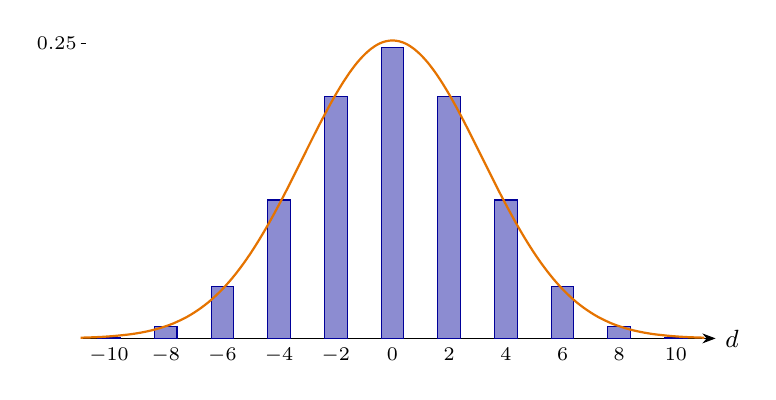
\begin{tikzpicture}[x=0.36cm,y=15.0cm,>=Stealth]
\draw[->] (-11,0) -- (11.4,0) node[right]{\small $d$};
\filldraw[fill=cBar!45,draw=cBar] (-10.4,0) rectangle (-9.6,0.0010);
\node[below,font=\scriptsize] at (-10,0) {$-10$};
\filldraw[fill=cBar!45,draw=cBar] (-8.4,0) rectangle (-7.6,0.0098);
\node[below,font=\scriptsize] at (-8,0) {$-8$};
\filldraw[fill=cBar!45,draw=cBar] (-6.4,0) rectangle (-5.6,0.0439);
\node[below,font=\scriptsize] at (-6,0) {$-6$};
\filldraw[fill=cBar!45,draw=cBar] (-4.4,0) rectangle (-3.6,0.1172);
\node[below,font=\scriptsize] at (-4,0) {$-4$};
\filldraw[fill=cBar!45,draw=cBar] (-2.4,0) rectangle (-1.6,0.2051);
\node[below,font=\scriptsize] at (-2,0) {$-2$};
\filldraw[fill=cBar!45,draw=cBar] (-0.4,0) rectangle (0.4,0.2461);
\node[below,font=\scriptsize] at (0,0) {$0$};
\filldraw[fill=cBar!45,draw=cBar] (1.6,0) rectangle (2.4,0.2051);
\node[below,font=\scriptsize] at (2,0) {$2$};
\filldraw[fill=cBar!45,draw=cBar] (3.6,0) rectangle (4.4,0.1172);
\node[below,font=\scriptsize] at (4,0) {$4$};
\filldraw[fill=cBar!45,draw=cBar] (5.6,0) rectangle (6.4,0.0439);
\node[below,font=\scriptsize] at (6,0) {$6$};
\filldraw[fill=cBar!45,draw=cBar] (7.6,0) rectangle (8.4,0.0098);
\node[below,font=\scriptsize] at (8,0) {$8$};
\filldraw[fill=cBar!45,draw=cBar] (9.6,0) rectangle (10.4,0.0010);
\node[below,font=\scriptsize] at (10,0) {$10$};
\draw[cGauss,thick] plot[smooth] coordinates {(-11.00,0.0006) (-10.75,0.0008) (-10.50,0.0010) (-10.25,0.0013) (-10.00,0.0017) (-9.75,0.0022) (-9.50,0.0028) (-9.25,0.0035) (-9.00,0.0044) (-8.75,0.0055) (-8.50,0.0068) (-8.25,0.0084) (-8.00,0.0103) (-7.75,0.0125) (-7.50,0.0152) (-7.25,0.0182) (-7.00,0.0218) (-6.75,0.0259) (-6.50,0.0305) (-6.25,0.0358) (-6.00,0.0417) (-5.75,0.0483) (-5.50,0.0556) (-5.25,0.0636) (-5.00,0.0723) (-4.75,0.0817) (-4.50,0.0917) (-4.25,0.1023) (-4.00,0.1134) (-3.75,0.1249) (-3.50,0.1368) (-3.25,0.1488) (-3.00,0.1609) (-2.75,0.1729) (-2.50,0.1846) (-2.25,0.1959) (-2.00,0.2066) (-1.75,0.2165) (-1.50,0.2255) (-1.25,0.2334) (-1.00,0.2400) (-0.75,0.2453) (-0.50,0.2492) (-0.25,0.2515) (0.00,0.2523) (0.25,0.2515) (0.50,0.2492) (0.75,0.2453) (1.00,0.2400) (1.25,0.2334) (1.50,0.2255) (1.75,0.2165) (2.00,0.2066) (2.25,0.1959) (2.50,0.1846) (2.75,0.1729) (3.00,0.1609) (3.25,0.1488) (3.50,0.1368) (3.75,0.1249) (4.00,0.1134) (4.25,0.1023) (4.50,0.0917) (4.75,0.0817) (5.00,0.0723) (5.25,0.0636) (5.50,0.0556) (5.75,0.0483) (6.00,0.0417) (6.25,0.0358) (6.50,0.0305) (6.75,0.0259) (7.00,0.0218) (7.25,0.0182) (7.50,0.0152) (7.75,0.0125) (8.00,0.0103) (8.25,0.0084) (8.50,0.0068) (8.75,0.0055) (9.00,0.0044) (9.25,0.0035) (9.50,0.0028) (9.75,0.0022) (10.00,0.0017) (10.25,0.0013) (10.50,0.0010) (10.75,0.0008) (11.00,0.0006)};
\draw (-11,0.25) -- (-10.8,0.25) node[left,font=\scriptsize] {$0.25$};
\end{tikzpicture}
}

\newcommand{\FigPascal}{%
\begin{tikzpicture}[x=0.5cm,y=0.62cm,>=Stealth]
\node[font=\small] (n0_10) at (0,0) {$1$};
\node[font=\scriptsize,gray] at (-10.5,0) {$N=0$};
\node[font=\small] (n1_9) at (-1,-1) {$1$};
\node[font=\small] (n1_11) at (1,-1) {$1$};
\node[font=\scriptsize,gray] at (-10.5,-1) {$N=1$};
\node[font=\small] (n2_8) at (-2,-2) {$1$};
\node[font=\small] (n2_10) at (0,-2) {$2$};
\node[font=\small] (n2_12) at (2,-2) {$1$};
\node[font=\scriptsize,gray] at (-10.5,-2) {$N=2$};
\node[font=\small] (n3_7) at (-3,-3) {$1$};
\node[font=\small] (n3_9) at (-1,-3) {$3$};
\node[font=\small] (n3_11) at (1,-3) {$3$};
\node[font=\small] (n3_13) at (3,-3) {$1$};
\node[font=\scriptsize,gray] at (-10.5,-3) {$N=3$};
\node[font=\small] (n4_6) at (-4,-4) {$1$};
\node[font=\small] (n4_8) at (-2,-4) {$4$};
\node[font=\small] (n4_10) at (0,-4) {$6$};
\node[font=\small] (n4_12) at (2,-4) {$4$};
\node[font=\small] (n4_14) at (4,-4) {$1$};
\node[font=\scriptsize,gray] at (-10.5,-4) {$N=4$};
\node[font=\small] (n5_5) at (-5,-5) {$1$};
\node[font=\small] (n5_7) at (-3,-5) {$5$};
\node[font=\small,text=cBar] (n5_9) at (-1,-5) {$10$};
\node[font=\small,text=cBar] (n5_11) at (1,-5) {$10$};
\node[font=\small] (n5_13) at (3,-5) {$5$};
\node[font=\small] (n5_15) at (5,-5) {$1$};
\node[font=\scriptsize,gray] at (-10.5,-5) {$N=5$};
\node[font=\small] (n6_4) at (-6,-6) {$1$};
\node[font=\small] (n6_6) at (-4,-6) {$6$};
\node[font=\small] (n6_8) at (-2,-6) {$15$};
\node[font=\small\bfseries,text=cWrong] (n6_10) at (0,-6) {$20$};
\node[font=\small] (n6_12) at (2,-6) {$15$};
\node[font=\small] (n6_14) at (4,-6) {$6$};
\node[font=\small] (n6_16) at (6,-6) {$1$};
\node[font=\scriptsize,gray] at (-10.5,-6) {$N=6$};
\node[font=\small] (n7_3) at (-7,-7) {$1$};
\node[font=\small] (n7_5) at (-5,-7) {$7$};
\node[font=\small] (n7_7) at (-3,-7) {$21$};
\node[font=\small] (n7_9) at (-1,-7) {$35$};
\node[font=\small] (n7_11) at (1,-7) {$35$};
\node[font=\small] (n7_13) at (3,-7) {$21$};
\node[font=\small] (n7_15) at (5,-7) {$7$};
\node[font=\small] (n7_17) at (7,-7) {$1$};
\node[font=\scriptsize,gray] at (-10.5,-7) {$N=7$};
\node[font=\small] (n8_2) at (-8,-8) {$1$};
\node[font=\small] (n8_4) at (-6,-8) {$8$};
\node[font=\small] (n8_6) at (-4,-8) {$28$};
\node[font=\small] (n8_8) at (-2,-8) {$56$};
\node[font=\small] (n8_10) at (0,-8) {$70$};
\node[font=\small] (n8_12) at (2,-8) {$56$};
\node[font=\small] (n8_14) at (4,-8) {$28$};
\node[font=\small] (n8_16) at (6,-8) {$8$};
\node[font=\small] (n8_18) at (8,-8) {$1$};
\node[font=\scriptsize,gray] at (-10.5,-8) {$N=8$};
\draw[->,cBar,thick] (n5_9) -- (n6_10);
\draw[->,cBar,thick] (n5_11) -- (n6_10);
\end{tikzpicture}
}

\newcommand{\FigDiffusion}{%
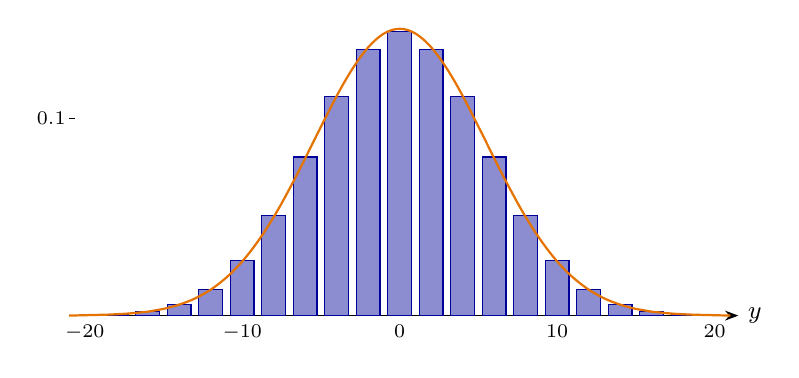
\begin{tikzpicture}[x=0.2cm,y=25.0cm,>=Stealth]
\draw[->] (-21,0) -- (21.5,0) node[right]{\small $y$};
\filldraw[fill=cBar!45,draw=cBar] (-20.75,0) rectangle (-19.25,0.0001);
\filldraw[fill=cBar!45,draw=cBar] (-18.75,0) rectangle (-17.25,0.0006);
\filldraw[fill=cBar!45,draw=cBar] (-16.75,0) rectangle (-15.25,0.0019);
\filldraw[fill=cBar!45,draw=cBar] (-14.75,0) rectangle (-13.25,0.0055);
\filldraw[fill=cBar!45,draw=cBar] (-12.75,0) rectangle (-11.25,0.0133);
\filldraw[fill=cBar!45,draw=cBar] (-10.75,0) rectangle (-9.25,0.0280);
\filldraw[fill=cBar!45,draw=cBar] (-8.75,0) rectangle (-7.25,0.0509);
\filldraw[fill=cBar!45,draw=cBar] (-6.75,0) rectangle (-5.25,0.0806);
\filldraw[fill=cBar!45,draw=cBar] (-4.75,0) rectangle (-3.25,0.1115);
\filldraw[fill=cBar!45,draw=cBar] (-2.75,0) rectangle (-1.25,0.1354);
\filldraw[fill=cBar!45,draw=cBar] (-0.75,0) rectangle (0.75,0.1445);
\filldraw[fill=cBar!45,draw=cBar] (1.25,0) rectangle (2.75,0.1354);
\filldraw[fill=cBar!45,draw=cBar] (3.25,0) rectangle (4.75,0.1115);
\filldraw[fill=cBar!45,draw=cBar] (5.25,0) rectangle (6.75,0.0806);
\filldraw[fill=cBar!45,draw=cBar] (7.25,0) rectangle (8.75,0.0509);
\filldraw[fill=cBar!45,draw=cBar] (9.25,0) rectangle (10.75,0.0280);
\filldraw[fill=cBar!45,draw=cBar] (11.25,0) rectangle (12.75,0.0133);
\filldraw[fill=cBar!45,draw=cBar] (13.25,0) rectangle (14.75,0.0055);
\filldraw[fill=cBar!45,draw=cBar] (15.25,0) rectangle (16.75,0.0019);
\filldraw[fill=cBar!45,draw=cBar] (17.25,0) rectangle (18.75,0.0006);
\filldraw[fill=cBar!45,draw=cBar] (19.25,0) rectangle (20.75,0.0001);
\node[below,font=\scriptsize] at (-20,0) {$-20$};
\node[below,font=\scriptsize] at (-10,0) {$-10$};
\node[below,font=\scriptsize] at (0,0) {$0$};
\node[below,font=\scriptsize] at (10,0) {$10$};
\node[below,font=\scriptsize] at (20,0) {$20$};
\draw[cGauss,thick] plot[smooth] coordinates {(-21.0,0.0001) (-20.5,0.0001) (-20.0,0.0002) (-19.5,0.0003) (-19.0,0.0004) (-18.5,0.0005) (-18.0,0.0007) (-17.5,0.0009) (-17.0,0.0012) (-16.5,0.0016) (-16.0,0.0020) (-15.5,0.0027) (-15.0,0.0034) (-14.5,0.0044) (-14.0,0.0056) (-13.5,0.0070) (-13.0,0.0087) (-12.5,0.0108) (-12.0,0.0132) (-11.5,0.0161) (-11.0,0.0194) (-10.5,0.0232) (-10.0,0.0275) (-9.5,0.0324) (-9.0,0.0378) (-8.5,0.0437) (-8.0,0.0501) (-7.5,0.0570) (-7.0,0.0644) (-6.5,0.0720) (-6.0,0.0799) (-5.5,0.0880) (-5.0,0.0960) (-4.5,0.1039) (-4.0,0.1116) (-3.5,0.1188) (-3.0,0.1254) (-2.5,0.1313) (-2.0,0.1363) (-1.5,0.1403) (-1.0,0.1433) (-0.5,0.1451) (0.0,0.1457) (0.5,0.1451) (1.0,0.1433) (1.5,0.1403) (2.0,0.1363) (2.5,0.1313) (3.0,0.1254) (3.5,0.1188) (4.0,0.1116) (4.5,0.1039) (5.0,0.0960) (5.5,0.0880) (6.0,0.0799) (6.5,0.0720) (7.0,0.0644) (7.5,0.0570) (8.0,0.0501) (8.5,0.0437) (9.0,0.0378) (9.5,0.0324) (10.0,0.0275) (10.5,0.0232) (11.0,0.0194) (11.5,0.0161) (12.0,0.0132) (12.5,0.0108) (13.0,0.0087) (13.5,0.0070) (14.0,0.0056) (14.5,0.0044) (15.0,0.0034) (15.5,0.0027) (16.0,0.0020) (16.5,0.0016) (17.0,0.0012) (17.5,0.0009) (18.0,0.0007) (18.5,0.0005) (19.0,0.0004) (19.5,0.0003) (20.0,0.0002) (20.5,0.0001) (21.0,0.0001)};
\draw (-21,0.1) -- (-20.6,0.1) node[left,font=\scriptsize] {$0.1$};
\end{tikzpicture}
}

\newcommand{\FigChiPower}{%
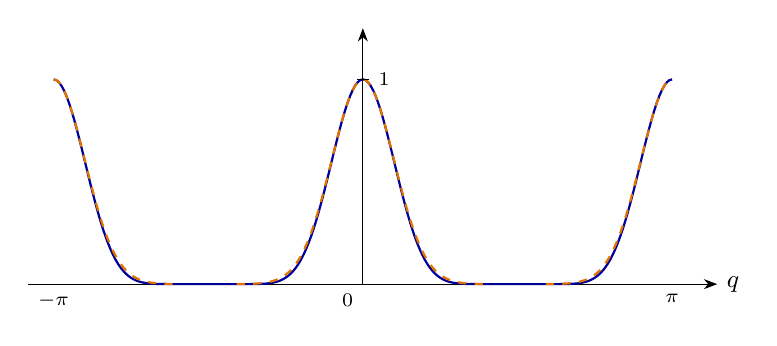
\begin{tikzpicture}[x=1.25cm,y=2.6cm,>=Stealth]
\draw[->] (-3.4,0) -- (3.6,0) node[right]{\small $q$};
\draw[->] (0,0) -- (0,1.25);
\draw[cBar,thick] plot coordinates {(-3.1416,1.0000) (-3.1154,0.9966) (-3.0892,0.9864) (-3.0631,0.9696) (-3.0369,0.9465) (-3.0107,0.9177) (-2.9845,0.8835) (-2.9583,0.8446) (-2.9322,0.8018) (-2.9060,0.7556) (-2.8798,0.7070) (-2.8536,0.6567) (-2.8274,0.6054) (-2.8013,0.5539) (-2.7751,0.5029) (-2.7489,0.4531) (-2.7227,0.4049) (-2.6965,0.3588) (-2.6704,0.3154) (-2.6442,0.2748) (-2.6180,0.2373) (-2.5918,0.2031) (-2.5656,0.1722) (-2.5395,0.1445) (-2.5133,0.1201) (-2.4871,0.0988) (-2.4609,0.0804) (-2.4347,0.0646) (-2.4086,0.0514) (-2.3824,0.0403) (-2.3562,0.0312) (-2.3300,0.0239) (-2.3038,0.0180) (-2.2777,0.0133) (-2.2515,0.0097) (-2.2253,0.0070) (-2.1991,0.0049) (-2.1729,0.0034) (-2.1468,0.0023) (-2.1206,0.0015) (-2.0944,0.0010) (-2.0682,0.0006) (-2.0420,0.0004) (-2.0159,0.0002) (-1.9897,0.0001) (-1.9635,0.0001) (-1.9373,0.0000) (-1.9111,0.0000) (-1.8850,0.0000) (-1.8588,0.0000) (-1.8326,0.0000) (-1.8064,0.0000) (-1.7802,0.0000) (-1.7541,0.0000) (-1.7279,0.0000) (-1.7017,0.0000) (-1.6755,0.0000) (-1.6493,0.0000) (-1.6232,0.0000) (-1.5970,0.0000) (-1.5708,0.0000) (-1.5446,0.0000) (-1.5184,0.0000) (-1.4923,0.0000) (-1.4661,0.0000) (-1.4399,0.0000) (-1.4137,0.0000) (-1.3875,0.0000) (-1.3614,0.0000) (-1.3352,0.0000) (-1.3090,0.0000) (-1.2828,0.0000) (-1.2566,0.0000) (-1.2305,0.0000) (-1.2043,0.0000) (-1.1781,0.0001) (-1.1519,0.0001) (-1.1257,0.0002) (-1.0996,0.0004) (-1.0734,0.0006) (-1.0472,0.0010) (-1.0210,0.0015) (-0.9948,0.0023) (-0.9687,0.0034) (-0.9425,0.0049) (-0.9163,0.0070) (-0.8901,0.0097) (-0.8639,0.0133) (-0.8378,0.0180) (-0.8116,0.0239) (-0.7854,0.0313) (-0.7592,0.0403) (-0.7330,0.0514) (-0.7069,0.0646) (-0.6807,0.0804) (-0.6545,0.0988) (-0.6283,0.1201) (-0.6021,0.1445) (-0.5760,0.1722) (-0.5498,0.2031) (-0.5236,0.2373) (-0.4974,0.2748) (-0.4712,0.3154) (-0.4451,0.3588) (-0.4189,0.4049) (-0.3927,0.4531) (-0.3665,0.5029) (-0.3403,0.5539) (-0.3142,0.6054) (-0.2880,0.6567) (-0.2618,0.7070) (-0.2356,0.7556) (-0.2094,0.8018) (-0.1833,0.8446) (-0.1571,0.8835) (-0.1309,0.9177) (-0.1047,0.9465) (-0.0785,0.9696) (-0.0524,0.9864) (-0.0262,0.9966) (-0.0000,1.0000) (0.0262,0.9966) (0.0524,0.9864) (0.0785,0.9696) (0.1047,0.9465) (0.1309,0.9177) (0.1571,0.8835) (0.1833,0.8446) (0.2094,0.8018) (0.2356,0.7556) (0.2618,0.7070) (0.2880,0.6567) (0.3142,0.6054) (0.3403,0.5539) (0.3665,0.5029) (0.3927,0.4531) (0.4189,0.4049) (0.4451,0.3588) (0.4712,0.3154) (0.4974,0.2748) (0.5236,0.2373) (0.5498,0.2031) (0.5760,0.1722) (0.6021,0.1445) (0.6283,0.1201) (0.6545,0.0988) (0.6807,0.0804) (0.7069,0.0646) (0.7330,0.0514) (0.7592,0.0403) (0.7854,0.0313) (0.8116,0.0239) (0.8378,0.0180) (0.8639,0.0133) (0.8901,0.0097) (0.9163,0.0070) (0.9425,0.0049) (0.9687,0.0034) (0.9948,0.0023) (1.0210,0.0015) (1.0472,0.0010) (1.0734,0.0006) (1.0996,0.0004) (1.1257,0.0002) (1.1519,0.0001) (1.1781,0.0001) (1.2043,0.0000) (1.2305,0.0000) (1.2566,0.0000) (1.2828,0.0000) (1.3090,0.0000) (1.3352,0.0000) (1.3614,0.0000) (1.3875,0.0000) (1.4137,0.0000) (1.4399,0.0000) (1.4661,0.0000) (1.4923,0.0000) (1.5184,0.0000) (1.5446,0.0000) (1.5708,0.0000) (1.5970,0.0000) (1.6232,0.0000) (1.6493,0.0000) (1.6755,0.0000) (1.7017,0.0000) (1.7279,0.0000) (1.7541,0.0000) (1.7802,0.0000) (1.8064,0.0000) (1.8326,0.0000) (1.8588,0.0000) (1.8850,0.0000) (1.9111,0.0000) (1.9373,0.0000) (1.9635,0.0001) (1.9897,0.0001) (2.0159,0.0002) (2.0420,0.0004) (2.0682,0.0006) (2.0944,0.0010) (2.1206,0.0015) (2.1468,0.0023) (2.1729,0.0034) (2.1991,0.0049) (2.2253,0.0070) (2.2515,0.0097) (2.2777,0.0133) (2.3038,0.0180) (2.3300,0.0239) (2.3562,0.0312) (2.3824,0.0403) (2.4086,0.0514) (2.4347,0.0646) (2.4609,0.0804) (2.4871,0.0988) (2.5133,0.1201) (2.5395,0.1445) (2.5656,0.1722) (2.5918,0.2031) (2.6180,0.2373) (2.6442,0.2748) (2.6704,0.3154) (2.6965,0.3588) (2.7227,0.4049) (2.7489,0.4531) (2.7751,0.5029) (2.8013,0.5539) (2.8274,0.6054) (2.8536,0.6567) (2.8798,0.7070) (2.9060,0.7556) (2.9322,0.8018) (2.9583,0.8446) (2.9845,0.8835) (3.0107,0.9177) (3.0369,0.9465) (3.0631,0.9696) (3.0892,0.9864) (3.1154,0.9966) (3.1416,1.0000)};
\draw[cGauss,thick,dashed] plot coordinates {(-1.2828,0.0003) (-1.2566,0.0004) (-1.2305,0.0005) (-1.2043,0.0007) (-1.1781,0.0010) (-1.1519,0.0013) (-1.1257,0.0018) (-1.0996,0.0024) (-1.0734,0.0031) (-1.0472,0.0042) (-1.0210,0.0054) (-0.9948,0.0071) (-0.9687,0.0092) (-0.9425,0.0118) (-0.9163,0.0150) (-0.8901,0.0190) (-0.8639,0.0239) (-0.8378,0.0299) (-0.8116,0.0371) (-0.7854,0.0458) (-0.7592,0.0560) (-0.7330,0.0681) (-0.7069,0.0822) (-0.6807,0.0986) (-0.6545,0.1174) (-0.6283,0.1389) (-0.6021,0.1632) (-0.5760,0.1904) (-0.5498,0.2206) (-0.5236,0.2539) (-0.4974,0.2902) (-0.4712,0.3295) (-0.4451,0.3714) (-0.4189,0.4159) (-0.3927,0.4625) (-0.3665,0.5108) (-0.3403,0.5604) (-0.3142,0.6105) (-0.2880,0.6606) (-0.2618,0.7099) (-0.2356,0.7576) (-0.2094,0.8031) (-0.1833,0.8454) (-0.1571,0.8839) (-0.1309,0.9179) (-0.1047,0.9466) (-0.0785,0.9696) (-0.0524,0.9864) (-0.0262,0.9966) (-0.0000,1.0000) (0.0262,0.9966) (0.0524,0.9864) (0.0785,0.9696) (0.1047,0.9466) (0.1309,0.9179) (0.1571,0.8839) (0.1833,0.8454) (0.2094,0.8031) (0.2356,0.7576) (0.2618,0.7099) (0.2880,0.6606) (0.3142,0.6105) (0.3403,0.5604) (0.3665,0.5108) (0.3927,0.4625) (0.4189,0.4159) (0.4451,0.3714) (0.4712,0.3295) (0.4974,0.2902) (0.5236,0.2539) (0.5498,0.2206) (0.5760,0.1904) (0.6021,0.1632) (0.6283,0.1389) (0.6545,0.1174) (0.6807,0.0986) (0.7069,0.0822) (0.7330,0.0681) (0.7592,0.0560) (0.7854,0.0458) (0.8116,0.0371) (0.8378,0.0299) (0.8639,0.0239) (0.8901,0.0190) (0.9163,0.0150) (0.9425,0.0118) (0.9687,0.0092) (0.9948,0.0071) (1.0210,0.0054) (1.0472,0.0042) (1.0734,0.0031) (1.0996,0.0024) (1.1257,0.0018) (1.1519,0.0013) (1.1781,0.0010) (1.2043,0.0007) (1.2305,0.0005) (1.2566,0.0004) (1.2828,0.0003)};
\draw[cGauss,thick,dashed] plot coordinates {(-3.1416,1.0000) (-3.1154,0.9966) (-3.0892,0.9864) (-3.0631,0.9696) (-3.0369,0.9466) (-3.0107,0.9179) (-2.9845,0.8839) (-2.9583,0.8454) (-2.9322,0.8031) (-2.9060,0.7576) (-2.8798,0.7099) (-2.8536,0.6606) (-2.8274,0.6105) (-2.8013,0.5604) (-2.7751,0.5108) (-2.7489,0.4625) (-2.7227,0.4159) (-2.6965,0.3714) (-2.6704,0.3295) (-2.6442,0.2902) (-2.6180,0.2539) (-2.5918,0.2206) (-2.5656,0.1904) (-2.5395,0.1632) (-2.5133,0.1389) (-2.4871,0.1174) (-2.4609,0.0986) (-2.4347,0.0822) (-2.4086,0.0681) (-2.3824,0.0560) (-2.3562,0.0458) (-2.3300,0.0371) (-2.3038,0.0299) (-2.2777,0.0239) (-2.2515,0.0190) (-2.2253,0.0150) (-2.1991,0.0118) (-2.1729,0.0092) (-2.1468,0.0071) (-2.1206,0.0054) (-2.0944,0.0042) (-2.0682,0.0031) (-2.0420,0.0024) (-2.0159,0.0018) (-1.9897,0.0013) (-1.9635,0.0010) (-1.9373,0.0007) (-1.9111,0.0005) (-1.8850,0.0004) (-1.8588,0.0003)};
\draw[cGauss,thick,dashed] plot coordinates {(1.8588,0.0003) (1.8850,0.0004) (1.9111,0.0005) (1.9373,0.0007) (1.9635,0.0010) (1.9897,0.0013) (2.0159,0.0018) (2.0420,0.0024) (2.0682,0.0031) (2.0944,0.0042) (2.1206,0.0054) (2.1468,0.0071) (2.1729,0.0092) (2.1991,0.0118) (2.2253,0.0150) (2.2515,0.0190) (2.2777,0.0239) (2.3038,0.0299) (2.3300,0.0371) (2.3562,0.0458) (2.3824,0.0560) (2.4086,0.0681) (2.4347,0.0822) (2.4609,0.0986) (2.4871,0.1174) (2.5133,0.1389) (2.5395,0.1632) (2.5656,0.1904) (2.5918,0.2206) (2.6180,0.2539) (2.6442,0.2902) (2.6704,0.3295) (2.6965,0.3714) (2.7227,0.4159) (2.7489,0.4625) (2.7751,0.5108) (2.8013,0.5604) (2.8274,0.6105) (2.8536,0.6606) (2.8798,0.7099) (2.9060,0.7576) (2.9322,0.8031) (2.9583,0.8454) (2.9845,0.8839) (3.0107,0.9179) (3.0369,0.9466) (3.0631,0.9696) (3.0892,0.9864) (3.1154,0.9966) (3.1416,1.0000)};
\node[below,font=\scriptsize] at (-3.1416,0) {$-\pi$};
\node[below,font=\scriptsize] at (3.1416,0) {$\pi$};
\node[below left,font=\scriptsize] at (0,0) {$0$};
\draw (-0.06,1) -- (0.06,1) node[right,font=\scriptsize] {$1$};
\end{tikzpicture}
}

\newcommand{\FigContour}{%
\begin{tikzpicture}[x=4.0cm,y=4.0cm,>=Stealth]
\draw[->] (-0.45,0) -- (0.75,0) node[right]{\small $\mathrm{Re}\,z$};
\draw[->] (0,-0.45) -- (0,0.5) node[above]{\small $\mathrm{Im}\,z$};
\draw[cExact,thick,postaction={decorate},decoration={markings,mark=at position 0.15 with {\arrow{Stealth}}}] (0,0) circle (0.25);
\node[cExact,font=\scriptsize] at (-0.2,0.28) {$|z|=\tfrac14$};
\draw[cWrong,thick] (0.47,-0.03) -- (0.53,0.03) (0.47,0.03) -- (0.53,-0.03);
\node[cWrong,above,font=\scriptsize] at (0.5,0.03) {極點 $z=\tfrac12$};
\fill (0,0) circle (0.6pt);
\end{tikzpicture}
}

\newcommand{\FigSaddle}{%
\begin{tikzpicture}[>=Stealth]
\begin{scope}[xshift=-8.4cm,x=14cm,y=2.4cm]
\draw[->] (0.6,0) -- (0.99,0) node[right]{\small $x$};
\draw[->] (0.6,0) -- (0.6,1.95);
\draw[cBar,thick] plot[smooth] coordinates {(0.6200,1.3308) (0.6242,1.2626) (0.6285,1.1987) (0.6328,1.1390) (0.6370,1.0831) (0.6412,1.0307) (0.6455,0.9815) (0.6498,0.9355) (0.6540,0.8923) (0.6583,0.8517) (0.6625,0.8136) (0.6667,0.7778) (0.6710,0.7441) (0.6753,0.7125) (0.6795,0.6827) (0.6837,0.6547) (0.6880,0.6284) (0.6923,0.6035) (0.6965,0.5802) (0.7007,0.5581) (0.7050,0.5374) (0.7093,0.5178) (0.7135,0.4994) (0.7177,0.4820) (0.7220,0.4656) (0.7262,0.4501) (0.7305,0.4356) (0.7348,0.4218) (0.7390,0.4089) (0.7432,0.3967) (0.7475,0.3853) (0.7518,0.3745) (0.7560,0.3643) (0.7602,0.3548) (0.7645,0.3458) (0.7688,0.3374) (0.7730,0.3296) (0.7772,0.3223) (0.7815,0.3154) (0.7857,0.3091) (0.7900,0.3032) (0.7943,0.2977) (0.7985,0.2927) (0.8028,0.2881) (0.8070,0.2840) (0.8113,0.2802) (0.8155,0.2769) (0.8197,0.2740) (0.8240,0.2715) (0.8282,0.2694) (0.8325,0.2678) (0.8367,0.2665) (0.8410,0.2657) (0.8453,0.2654) (0.8495,0.2655) (0.8538,0.2662) (0.8580,0.2673) (0.8622,0.2691) (0.8665,0.2714) (0.8708,0.2744) (0.8750,0.2780) (0.8793,0.2825) (0.8835,0.2878) (0.8878,0.2941) (0.8920,0.3014) (0.8962,0.3100) (0.9005,0.3199) (0.9047,0.3315) (0.9090,0.3449) (0.9133,0.3606) (0.9175,0.3788) (0.9218,0.4002) (0.9260,0.4254) (0.9303,0.4553) (0.9345,0.4911) (0.9387,0.5342) (0.9430,0.5870) (0.9473,0.6523) (0.9515,0.7345) (0.9558,0.8402) (0.9600,0.9793)};
\draw[dashed,gray] (0.8462,0) -- (0.8462,0.2654);
\fill[cWrong] (0.8462,0.2654) circle (1.6pt);
\node[below,font=\scriptsize] at (0.8462,0) {$z^*=\tfrac{11}{13}$};
\node[below,font=\scriptsize] at (0.7,0) {$0.7$};
\node[below,font=\scriptsize] at (0.95,0) {$0.95$};
\draw (0.6,1) -- (0.607,1) node[left,font=\scriptsize] {$1000$};
\node[font=\small] at (0.79,2.1) {沿實軸：谷};
\end{scope}
\begin{scope}[xshift=9.4cm,x=16cm,y=14cm]
\draw[->] (-0.16,0) -- (0.17,0) node[right]{\small $y$};
\draw[->] (0,0) -- (0,0.33);
\draw[cGauss,thick] plot[smooth] coordinates {(-0.1500,0.1148) (-0.1462,0.1186) (-0.1425,0.1225) (-0.1387,0.1265) (-0.1350,0.1306) (-0.1313,0.1348) (-0.1275,0.1391) (-0.1237,0.1434) (-0.1200,0.1479) (-0.1162,0.1524) (-0.1125,0.1570) (-0.1087,0.1617) (-0.1050,0.1665) (-0.1012,0.1713) (-0.0975,0.1761) (-0.0938,0.1810) (-0.0900,0.1859) (-0.0862,0.1908) (-0.0825,0.1957) (-0.0787,0.2005) (-0.0750,0.2054) (-0.0712,0.2102) (-0.0675,0.2149) (-0.0638,0.2196) (-0.0600,0.2241) (-0.0562,0.2285) (-0.0525,0.2327) (-0.0488,0.2368) (-0.0450,0.2407) (-0.0413,0.2444) (-0.0375,0.2478) (-0.0338,0.2510) (-0.0300,0.2539) (-0.0262,0.2565) (-0.0225,0.2588) (-0.0187,0.2608) (-0.0150,0.2624) (-0.0113,0.2637) (-0.0075,0.2646) (-0.0038,0.2652) (0.0000,0.2654) (0.0038,0.2652) (0.0075,0.2646) (0.0113,0.2637) (0.0150,0.2624) (0.0188,0.2608) (0.0225,0.2588) (0.0262,0.2565) (0.0300,0.2539) (0.0338,0.2510) (0.0375,0.2478) (0.0412,0.2444) (0.0450,0.2407) (0.0487,0.2368) (0.0525,0.2327) (0.0562,0.2285) (0.0600,0.2241) (0.0637,0.2196) (0.0675,0.2149) (0.0713,0.2102) (0.0750,0.2054) (0.0788,0.2005) (0.0825,0.1957) (0.0862,0.1908) (0.0900,0.1859) (0.0938,0.1810) (0.0975,0.1761) (0.1012,0.1713) (0.1050,0.1665) (0.1087,0.1617) (0.1125,0.1570) (0.1162,0.1524) (0.1200,0.1479) (0.1237,0.1434) (0.1275,0.1391) (0.1313,0.1348) (0.1350,0.1306) (0.1387,0.1265) (0.1425,0.1225) (0.1463,0.1186) (0.1500,0.1148)};
\fill[cWrong] (0,0.2654) circle (1.6pt);
\node[below,font=\scriptsize] at (-0.15,0) {$-0.15$};
\node[below,font=\scriptsize] at (0.15,0) {$0.15$};
\draw (-0.004,0.1) -- (0.004,0.1) node[left=3pt,font=\scriptsize] {$100$};
\node[font=\small] at (0,0.36) {沿 $z=z^*+iy$：峰};
\end{scope}
\end{tikzpicture}
}

\newcommand{\TabErrata}{%
\begin{tabular}{@{}lll@{}}
\toprule
位置 & 書上 & 應為\\
\midrule
p. 6，(1.13) 前 & 每步位移的平方叫 $l$ & $l^2$\\
p. 8，(1.20) 前 & $x=N-2m$ & $x=l(2m-N)$（奇數次動差為 0，不影響結果）\\
p. 8--9，(1.22)(1.23) & 右邊沒有 $e^{Ny/2}$ & 乘上 $e^{Ny/2}$（$y=0$ 時等於 1）\\
p. 11，(1.34)(1.36) & $\exp[N(\ln N-N)]$ & $\exp[N\ln N-N]$\\
p. 12，(1.37) & $+\tfrac12\ln(2\pi n)$、$+\tfrac12\ln(2\pi(N-n))$ & 兩項都是 $-$\\
p. 12，(1.38) & $+\tfrac12(2m/N)^2$ & $-\tfrac12(2m/N)^2$\\
p. 12，(1.39)(1.40) & $n$；$-\tfrac12\ln 2\pi N$；$2^N/\sqrt{2\pi N}$ & $2m=d/l$；$-\tfrac12\ln\tfrac{\pi N}{2}$；$2\cdot2^N/\sqrt{2\pi N}$\\
p. 14，(1.48) & $\exp\big((x-y)^2/2l^2N\big)$ & $\exp\big(-(x-y)^2/2l^2N\big)$，$\alpha=1/\sqrt{2\pi l^2}$\\
p. 16，(1.54) 後 & 上下限換成 $\pm\infty$ 誤差可忽略 & 還要加 $q=\pm\pi/l$ 的鞍點（因子 2 或 0）\\
p. 17，(1.58) 後 & $N!\,d^N/dz^N$ & $\tfrac1{N!}\,d^N/dz^N$\\
p. 20，練習 1.7 & $d^4=3(d_N^2)^2$ & $\overline{d^4}=3N^2-2N\approx3(\overline{d^2})^2$\\
p. 21，(1:S-9) & $\exp(N|p''|\cdots)$ & $\exp(-\tfrac N2|p''|\cdots)$\\
p. 23，(1:S-15) & 前因子 $\tfrac1{2\pi}$ & $\tfrac1{\sqrt{2\pi}}$\\
\bottomrule
\end{tabular}
}


\section{技巧入門：最簡單的隨機漫步（第 1 章）}

\begin{keybox}[先看這裡]
這一章只研究一種漫步：\textbf{一維、每步長 $l$、向左向右的機率各 $\tfrac12$、每一步和以前無關}。作者說這是全書的「序曲」：
後面要用的工具在這裡先各露一次臉——
\begin{center}
\small
\begin{tabular}{@{}ll@{}}
數路線 & 二項式係數、奇偶性（1.1 節）\\
平均與動差 & 系綜平均、$\avg{x^2}=Nl^2$、用生成函數「微分」出所有動差（1.2 節）\\
大 $N$ 的近似 & Stirling 公式、二項分布 → 高斯（1.3 節）\\
連續極限 & 遞迴關係、Pascal 三角形、擴散方程（1.4 節）\\
生成函數 & 傅立葉表示、$g(z,q)=1/(1-z\chi(q))$、Cauchy 積分、奇點（1.5 節）\\
漸近分析 & 最陡下降法（鞍點法）（1.6 節）
\end{tabular}
\end{center}
\textbf{記號}：步長 $l$（例子裡都取 $l=1$）；步數 $N$；$N$ 步裡向右（正面）的步數 $n$（書上有時寫 $m$）；
終點離起點的距離 $d$（向右為正）；第 $j$ 步的位移 $\Delta_j=\pm l$；上橫線 $\avg{\,\cdot\,}$ 表示對所有可能的走法取平均。

\textbf{全章的主例}：擲十次硬幣得到 \coinH\coinT\coinH\coinH\coinT\coinH\coinT\coinT\coinH\coinH（6 正 4 反）。
\end{keybox}

% =====================================================================
\subsection{最簡單的漫步：擲硬幣決定方向}
\bk{pp.~1--5}\anim{W101、W102}

\paragraph{直觀。}
一個人站在一條直線上。每一步之前擲一枚硬幣：正面就向右走一步，反面就向左走一步，步長都是 $l$。
因為硬幣公正，向左向右一樣可能——這叫\textbf{無偏}（unbiased）漫步。
書上提了三個「真實世界」的例子：分子在細管裡因熱運動而擴散；一條高分子鏈，每一節只有兩種取向；
以及擲硬幣的賭局（de Moivre 解「賭徒破產問題」時就用到了這個模型）。

\paragraph{主例。}
擲十次得到 \coinH\coinT\coinH\coinH\coinT\coinH\coinT\coinT\coinH\coinH，每一步之後的位置依序是
$0,1,0,1,2,1,2,1,0,1,2$（圖 \ref{fig:mainwalk}）。最後停在 $d=2$。

\begin{figure}[H]
\centering
\FigMainWalk
\caption{主例：十次擲幣的走法圖。橫軸是步數、縱軸是位置；上面一排是每一步擲出的硬幣。}
\label{fig:mainwalk}
\end{figure}

\paragraph{終點和正面數。}
如果 $N$ 次裡有 $n$ 次正面、$N-n$ 次反面，那麼向右 $n$ 步、向左 $N-n$ 步，終點是
\begin{equation}
d=nl-(N-n)l=l(2n-N). \tag{1.1}
\end{equation}
反過來，由終點可以讀出正面數與反面數：
\begin{equation}
n=\frac12\Big(\frac dl+N\Big),\qquad N-n=\frac12\Big(N-\frac dl\Big). \tag{1.2--1.3}
\end{equation}
\textbf{例}：主例 $N=10$、$n=6$，$d=1\cdot(12-10)=2$；反過來 $n=\frac12(2+10)=6$。\par
\textbf{奇偶性}：$d/l=2n-N$ 和 $N$ 同奇偶。走 10 步只能停在偶數位置；走 3 步只能停在奇數位置。這個看似無聊的事實，到 1.3 節與 1.5 節會變成一個「因子 2」。

\paragraph{一條指定路線的機率。}
每次擲幣都和之前無關（獨立），每次的機率都是 $\tfrac12$，所以一條\emph{指定}的正反序列（例如主例）出現的機率是
$(\tfrac12)^N$。$N=10$ 時是 $1/1024$。\emph{每一條}路線都一樣可能——不一樣的是「有幾條路線通往同一個終點」。

\paragraph{數路線：二項式係數。}
$N$ 次裡恰好 $n$ 次正面的序列有幾個？先看 $N=3$（表 \ref{tab:threecoins}）：

\begin{table}[H]
\centering
\TabThreeCoins
\caption{$N=3$ 的全部 $2^3=8$ 個序列，依正面數分組。書上 Fig.~1.2 畫的就是第二列的三個。}
\label{tab:threecoins}
\end{table}

書上的「洗牌論證」\bk{p.~3}：把書上 Fig.~1.1 的三枚硬幣「正反正」排成一列，標成 正$_1$、反、正$_2$。
三枚不同的硬幣排成一列有 $3!=6$ 種排法；但兩個正面互換看起來一樣，所以每個「看得見的序列」被數了 $2!$ 次，
真正不同的只有 $3!/2!=3$ 種。一般地，把 $n$ 個正面、$N-n$ 個反面排成一列的方法數是
\begin{equation}
\binom Nn=\frac{N!}{n!\,(N-n)!}, \tag{1.4}
\end{equation}
所以恰好 $n$ 次正面的機率是
\begin{equation}
\frac1{2^N}\,\frac{N!}{n!\,(N-n)!}. \tag{1.5}
\end{equation}
把 (1.2) 代進去，換成終點 $d$ 的語言：走 $N$ 步停在 $d$ 的走法數與機率是
\begin{equation}
C(N,d)=\frac{N!}{\big(\frac{N+d/l}{2}\big)!\,\big(\frac{N-d/l}{2}\big)!},\qquad
P(N,d)=\frac{1}{2^N}C(N,d). \tag{1.6--1.7}
\end{equation}
$P(N,d)$ 叫做\textbf{二項分布}。$d$ 和 $N$ 不同奇偶時 $C(N,d)=0$。

\textbf{例（$N=4$）}：$d=-4,-2,0,2,4$ 的走法數是 $1,4,6,4,1$，加起來 $16=2^4$；停在原點的機率 $6/16$。\par
\textbf{例（主例 $N=10$）}：停在原點的走法 $C(10,0)=\frac{10!}{5!\,5!}=252$ 種，機率 $252/1024=63/256\approx0.2461$；
主例的終點 $d=2$ 有 $C(10,2)=210$ 種走法。完整的分布見表 \ref{tab:tendist}（$d<0$ 的一半對稱）。

\begin{table}[H]
\centering
\small
\TabTenDist
\caption{$N=10$ 的終點分布（只列 $d\ge0$）。最後一列是 1.3 節的高斯近似（含奇偶性的因子 2）。}
\label{tab:tendist}
\end{table}

\paragraph{練習。}
\begin{enumerate}[label=(\alph*)]
\item 走 5 步停在 $d=1$ 的走法有幾種？機率多少？\\
  \textbf{答}：$n=\frac12(1+5)=3$，$C(5,1)=\binom53=10$，機率 $10/32=5/16$。
\item 走 6 步，最可能停在哪裡？機率多少？\\
  \textbf{答}：分布是 $1,6,15,20,15,6,1$（$d=-6,\dots,6$），最可能是 $d=0$，機率 $20/64=5/16$。
\item （書上練習 1.1）如果硬幣不公正，正面的機率是 $p\ne\tfrac12$（每次都一樣），(1.5) 要怎麼改？\\
  \textbf{答}：一條有 $n$ 個正面的指定序列機率是 $p^n(1-p)^{N-n}$，所以 $P(n)=\binom Nn p^n(1-p)^{N-n}$。
  例：$N=3$、$p=\tfrac23$，$n=0,1,2,3$ 的機率是 $\tfrac1{27},\tfrac6{27},\tfrac{12}{27},\tfrac8{27}$（加起來 1）；
  $N=10$、$p=\tfrac23$ 時最可能 $n=7$，機率 $\binom{10}{7}\frac{2^7}{3^{10}}\approx0.2601$。這就是第 5 章「有偏向的漫步」。
\item 走 10 步能不能停在 $d=3$？\\
  \textbf{答}：不能。$d$ 必須和 $N$ 同奇偶，$C(10,3)=0$。
\end{enumerate}

% =====================================================================
\subsection{平均位置與均方位移}
\bk{pp.~5--10}\anim{W103、W104、W105}

\subsubsection*{平均位置是 0}
想像 $M$ 個人同時出發、「鎖步」前進（每個人各擲自己的硬幣）。第 $i$ 個人停在 $x_i$，平均位置
\begin{equation}
\bar x=\frac1M\sum_{i=1}^Mx_i=\frac1M\sum_x x\,w(x), \tag{1.8--1.9}
\end{equation}
其中 $w(x)$ 是停在 $x$ 的人數。因為向左向右一樣可能，「平均來說」停在 $x$ 和停在 $-x$ 的人一樣多，$x\,w(x)$ 與 $-x\,w(-x)$ 抵消。

\textbf{例（有限的系綜）}：讓 20 個人各走 10 步（動畫 W103 用固定的亂數種子），終點加起來是 2，所以 $\bar x=2/20=0.1$——
不是剛好 0，因為 20 個人太少，抵消得不完美。書上說要做「超級平均」：對很多很多組系綜再平均，
等於直接對精確的分布平均：$\sum_dd\,C(10,d)=0$（分布左右對稱），所以 $\bar x=0$。

\subsubsection*{均方位移與 $\sqrt N$ 定律}
平均位置是 0，並不表示每個人都留在原地——上面那 20 個人的終點平方平均是 $63/5=12.6$，一點也不小。
所以改看\textbf{均方位移} $\avg{x^2}$。令第 $j$ 步的位移為 $\Delta_j=\pm l$，則
\begin{equation}
x=\sum_{j=1}^N\Delta_j,\qquad x^2=\Big(\sum_{j=1}^N\Delta_j\Big)^2. \tag{1.11, 1.10}
\end{equation}
把平方展開成 $N\times N$ 個乘積 $\Delta_j\Delta_k$（圖 \ref{fig:deltagrid}）：
\begin{equation}
\avg{x^2}=\sum_j\avg{\Delta_j^2}+\sum_{j\ne k}\avg{\Delta_j\Delta_k}
=\sum_j\avg{\Delta_j^2}+\sum_{j\ne k}\avg{\Delta_j}\times\avg{\Delta_k}. \tag{1.12}
\end{equation}
對角線上的 $N$ 格：$\Delta_j^2=l^2$，不管往哪走都一樣。對角線外的 $N(N-1)$ 格：兩步互相獨立，乘積的平均等於平均的乘積，而 $\avg{\Delta_j}=0$，
所以全部是 0。結論：
\begin{equation}
\avg{x^2}=Nl^2,\qquad \sqrt{\avg{x^2}}=l\sqrt N. \tag{1.13--1.14}
\end{equation}

\begin{figure}[H]
\centering
\FigDeltaGrid
\caption{$N=4$：$x^2=(\Delta_1+\cdots+\Delta_4)^2$ 展開成 16 格。黃色的對角格永遠是 $l^2$；灰色的 12 格平均是 0。}
\label{fig:deltagrid}
\end{figure}

\begin{errbox}[p.~6，(1.13) 前]
書上說「每一步位移的平方等於一個固定的數，我們叫它 $l$」；應該是 $l^2$（步長是 $l$）。
\end{errbox}

\textbf{例（直接核對）}：$N=4$ 的 16 條路線，終點平方加起來 $1\cdot16+4\cdot4+6\cdot0+4\cdot4+1\cdot16=64$，平均 $64/16=4=N$。\par
\textbf{$\sqrt N$ 定律}：走 100 步，平均只離家 $\sqrt{100}=10$ 步；走一萬步也只離家 100 步。動畫 W104 讓 2000 個人各走 100 步，
第 100 步時的樣本均方是 $98.922$（$\sqrt{\phantom{x}}\approx9.946$），和理論值 100 很接近。
距離是步數的\textbf{分數次方} $N^{1/2}$——書上說這種冪次律會貫穿全書（第 8--12 章的「標度」）。

\subsubsection*{例題：用生成函數算所有動差 \bk{pp.~7--9}}
\textbf{問題}：求 $\avg{x^n}$ 的一般公式。

\textbf{直接寫}：正面數為 $m$ 時位置是 $(2m-N)l$，機率是 (1.5)，所以
\begin{equation}
\avg{x^n}=\frac1{2^N}\sum_{m=0}^N\big((2m-N)l\big)^n\frac{N!}{m!\,(N-m)!}. \tag{1.15}
\end{equation}
要算 $\avg{x^4}$ 可以把 $(\sum\Delta_j)^4$ 展開（練習 1.3），但有更聰明的辦法——\textbf{生成函數}（generating function）。
二項式定理 $(1+w)^N=\sum_m\binom Nm w^m$（(1.16)）裡令 $w=e^y$、再除以 $2^N$：
\begin{equation}
g(y)\equiv\frac1{2^N}\left(1+e^y\right)^N=\frac1{2^N}\sum_{m=0}^N\frac{N!}{m!\,(N-m)!}e^{my}. \tag{1.17}
\end{equation}
$g(0)=1$（機率加起來是 1）。每對 $y$ 微分一次，右邊每一項就多乘一個 $m$：
\begin{equation}
g'(0)=\frac1{2^N}\sum_m\binom Nm m=\bar m,\qquad \avg{m^n}=g^{(n)}(0). \tag{1.18--1.19}
\end{equation}
\textbf{例}：$g'(y)=Ne^y(1+e^y)^{N-1}/2^N$，所以 $\bar m=N\cdot2^{N-1}/2^N=N/2$——平均一半是正面，理所當然。

要的是 $x=(2m-N)l$ 的動差，不是 $m$ 的。技巧：把 $g$ 寫成
\begin{equation}
g(y)=e^{Ny/2}\left(\frac{e^{y/2}+e^{-y/2}}{2}\right)^N=e^{Ny/2}\cosh(y/2)^N, \tag{1.21}
\end{equation}
「乘上 $N-2m$」等於對 $g$ 做運算子 $N-2\frac d{dy}$，而這個運算子作用在 $e^{Ny/2}F(y)$ 上剛好把 $e^{Ny/2}$ 吃掉：
$\big(N-2\frac d{dy}\big)\big(e^{Ny/2}F\big)=-2e^{Ny/2}F'$。反覆用 $n$ 次（練習 1.2），在 $y=0$ 取值，得到
\begin{equation}
\avg{x^n}=(-2l)^n\left.\frac{d^n}{dy^n}\cosh(y/2)^N\right|_{y=0}. \tag{1.24}
\end{equation}
（$x=-l(N-2m)$，多出來的 $(-1)^n$ 只影響奇數次動差，而它們都是 0。）

\begin{errbox}[p.~8--9，(1.22)(1.23)]
書上 $\big(N-2\frac d{dy}\big)^ng(y)=(-2)^n\frac{d^n}{dy^n}\cosh(y/2)^N$ 的右邊漏了因子 $e^{Ny/2}$；在 $y=0$ 它等於 1，所以 (1.24) 是對的。
另外 (1.20) 前「$x=N-2m$」應為 $x=l(2m-N)$。
\end{errbox}

$\cosh(y/2)=1+\frac{y^2}{8}+\frac{y^4}{384}+\cdots$，所以 $\cosh(y/2)^N=1+\frac{N}{8}y^2+\big(\frac{N}{384}+\binom N2\frac1{64}\big)y^4+\cdots$。
二階、四階導數在 0 的值是 $2!\cdot\frac N8=\frac N4$ 與 $4!\big(\frac{N}{384}+\frac{N(N-1)}{128}\big)=\frac{3N^2-2N}{16}$，乘上 $(-2l)^2=4l^2$、$(-2l)^4=16l^4$：
\begin{equation}
\avg{x^2}=Nl^2,\qquad \avg{x^4}=l^4N(3N-2). \tag{1.25--1.26}
\end{equation}
表 \ref{tab:moments} 列出小 $N$ 的值（$l=1$），每一格都用三種方法核對過：直接對分布加總、上面的公式、$\cosh$ 的冪級數。
主例 $N=10$：$\avg{x^2}=10$、$\avg{x^4}=280$、$\avg{x^6}=12160$。

\begin{table}[H]
\centering
\small
\TabMoments
\caption{前幾個偶數次動差（$l=1$；奇數次動差都是 0）。}
\label{tab:moments}
\end{table}

\paragraph{比值 → 3。}
$\avg{x^4}/(\avg{x^2})^2=3-2/N$，$N$ 很大時趨近 3（(1.27)，圖 \ref{fig:kurtosis}）。3 正是高斯分布的這個比值——下一節會看到，大 $N$ 時分布真的變成高斯。

\begin{figure}[H]
\centering
\FigKurtosis
\caption{$\avg{x^4}/(\avg{x^2})^2=3-2/N$：$N=1,\dots,10$ 依序是 $1,2,\tfrac73,\tfrac52,\tfrac{13}5,\tfrac83,\tfrac{19}7,\tfrac{11}4,\tfrac{25}9,\tfrac{14}5$。}
\label{fig:kurtosis}
\end{figure}

\paragraph{練習。}
\begin{enumerate}[label=(\alph*)]
\item （書上練習 1.2）用歸納法證明 $\big(N-2\frac d{dy}\big)^ng(y)=(-2)^ne^{Ny/2}\frac{d^n}{dy^n}\cosh(y/2)^N$。\\
  \textbf{答}：$n=0$ 是 (1.21)。設 $n$ 時成立，令 $F=\frac{d^n}{dy^n}\cosh(y/2)^N$，則
  $\big(N-2\frac d{dy}\big)\big[(-2)^ne^{Ny/2}F\big]=(-2)^n\big[Ne^{Ny/2}F-2\cdot\tfrac N2e^{Ny/2}F-2e^{Ny/2}F'\big]=(-2)^{n+1}e^{Ny/2}F'$。
\item （書上練習 1.3）直接用 $x=\sum_j\Delta_j$ 算 $\avg{x^3}$ 與 $\avg{x^4}$。\\
  \textbf{答}：$\avg{x^3}=\sum_{i,j,k}\avg{\Delta_i\Delta_j\Delta_k}$。不同的步獨立、$\avg{\Delta^{\text{奇數}}}=0$，所以只有「每個指標都出現偶數次」的項不為 0；
  三個指標做不到，$\avg{x^3}=0$。$\avg{x^4}$：四個指標全相同（$N$ 項，各為 $l^4$），或兩兩成對——配對方式 3 種、兩個不同的指標 $N(N-1)$ 種（$3N(N-1)$ 項，各為 $l^4$）。
  合計 $l^4(3N^2-2N)$，和 (1.26) 相同。例：$N=2$ 時 $2+6=8$。
\item 求 $\avg{x^6}$。\\
  \textbf{答}：同樣的數法（六個相同；四加二；三對）得 $l^6(15N^3-30N^2+16N)$；$N=1,2,3$ 時是 $1,32,183$，$N=10$ 時 12160。
\end{enumerate}

% =====================================================================
\subsection{Stirling 公式與高斯分布}
\bk{pp.~10--13}\anim{W106、W107}

公式 (1.6) 完全正確，但 $N$ 很大時不好用：$100!$ 有 158 位數。這一節用 \textbf{Stirling 公式}把階乘換成好算的函數。
\begin{equation}
\ln n!\approx n\ln\frac ne+\frac12\ln(2\pi n),\qquad\text{即}\quad n!\approx\sqrt{2\pi n}\,n^ne^{-n}. \tag{1.28}
\end{equation}

\subsubsection*{推導：階乘是一個積分 \bk{1.3.1 節}}
Gamma 函數 $\Gamma(x)=\int_0^\infty w^{x-1}e^{-w}dw$ 滿足 $N!=\Gamma(N+1)$（分部積分即可證），所以
\begin{equation}
N!=\int_0^\infty w^Ne^{-w}\,dw. \tag{1.29--1.31}
\end{equation}
被積函數 $w^Ne^{-w}$ 在 $w=N$ 有一個尖尖的峰（圖 \ref{fig:gamma}，$N=10$ 時峰高 $10^{10}e^{-10}\approx453\,999$）。令 $w=N+\delta$，把被積函數寫成 $e^{\text{指數}}$，指數在峰頂附近展開：
\begin{equation}
N\ln(N+\delta)-(N+\delta)=(N\ln N-N)-\frac{\delta^2}{2N}+O(\delta^3). \tag{1.33}
\end{equation}
所以被積函數 $\approx N^Ne^{-N}\,e^{-(w-N)^2/2N}$，一條高斯曲線（圖中虛線）。高斯曲線的面積是 $\sqrt{2\pi N}$ 乘上峰高：
\begin{equation}
N!\approx\sqrt{2\pi N}\,\exp\left[N\ln N-N\right]. \tag{1.34}
\end{equation}

\begin{figure}[H]
\centering
\FigGamma
\caption{書上 Fig.~1.3 的重現：$w^{10}e^{-w}$（實線，面積 $10!=3\,628\,800$）與近似它的高斯 $\exp[10\ln10-10-(w-10)^2/20]$（虛線，面積 $3\,598\,696$）。}
\label{fig:gamma}
\end{figure}

\begin{errbox}[p.~11，(1.34)(1.36)]
書上寫成 $\exp[N(\ln N-N)]$，應為 $\exp[N\ln N-N]=\exp[N(\ln N-1)]$。書上的數值 15.0961 是用正確的式子算的。
\end{errbox}

\textbf{例（書上 (1.35)(1.36)）}：$\ln10!=15.1044$，$\ln\big(\sqrt{20\pi}\,10^{10}e^{-10}\big)=15.0961$，相對誤差約 $5.5\times10^{-4}$；
$N=100$ 時相對誤差只剩約 $2.3\times10^{-6}$。表 \ref{tab:stirling} 直接比較 $n!$ 與 Stirling：比值大約是 $1+\frac1{12n}$，$n$ 越大越準。

\begin{table}[H]
\centering
\small
\TabStirling
\caption{$n!$ 與 Stirling 公式。}
\label{tab:stirling}
\end{table}

\subsubsection*{二項分布 → 高斯分布}
把 Stirling 公式代進 (1.4)。三個階乘各換一次：
\begin{equation}
\binom Nn\approx\exp\Big[N\ln\frac Ne+\tfrac12\ln(2\pi N)-n\ln\frac ne-\tfrac12\ln(2\pi n)-(N-n)\ln\frac{N-n}e-\tfrac12\ln\big(2\pi(N-n)\big)\Big]. \tag{1.37}
\end{equation}
令 $n=\frac N2+m$（$m\ll N$），用 $\ln\big(\frac N2+m\big)=\ln\frac N2+\frac{2m}N-\frac12\big(\frac{2m}N\big)^2+\cdots$（(1.38)）展開，整理後
\begin{equation}
\ln\binom Nn\approx N\ln2-\frac{(2m)^2}{2N}-\frac12\ln\frac{\pi N}{2},\qquad
\binom Nn\approx 2^N\sqrt{\frac2{\pi N}}\,e^{-(2m)^2/2N}. \tag{1.39--1.40}
\end{equation}
而 $2m=2n-N=d/l$。除以 $2^N$：
\[
P(N,d)\approx\frac{2}{\sqrt{2\pi N}}\exp\Big(-\frac{d^2}{2Nl^2}\Big)\quad(d\text{ 與 }N\text{ 同奇偶}).
\]

\begin{errbox}[p.~12，(1.37)--(1.40)]
(1.37) 後兩個 $\tfrac12\ln$ 項書上是「$+$」，應為「$-$」（它們來自分母的 $n!$ 與 $(N-n)!$）。(1.38) 第三項書上是 $+\frac12(2m/N)^2$，應為 $-$。
(1.39)(1.40) 書上把 $2m$ 寫成 $n$，常數項寫成 $-\frac12\ln2\pi N$、前因子寫成 $2^N/\sqrt{2\pi N}$——少了一個因子 2（見下面的「因子 2」）。
\end{errbox}

\paragraph{因子 2 從哪裡來？（奇偶性）}
書上的 (1.41) 是
\begin{equation}
\frac1{\sqrt{2\pi N}}\exp\Big(-\frac{d^2}{2Nl^2}\Big), \tag{1.41}
\end{equation}
它是 $u=d/l$ 的\textbf{機率密度}（$\int du=1$）。但 $d/l$ 只能取和 $N$ 同奇偶的值——每隔一格才有一根柱子，
每根柱子「代表」寬度為 2 的一段，所以柱高（真正的機率）＝ 2 × 密度。圖 \ref{fig:binomgauss} 與表 \ref{tab:tendist}：
$P(10,0)=0.2461$ 對 $2\times0.12616=0.2523$；$P(10,4)=0.1172$ 對 $0.1134$。即使只有 10 步，高斯已經很準。

\begin{figure}[H]
\centering
\FigBinomGauss
\caption{$N=10$ 的二項分布（柱子）與 $\frac{2}{\sqrt{20\pi}}e^{-d^2/20}$（曲線）。奇數位置沒有柱子。}
\label{fig:binomgauss}
\end{figure}

\textbf{例（$N=100$）}：$\ln\binom{100}{50}=66.7838$，近似式 (1.39) 給 $66.7863$；$\binom{100}{50}=1.0089\times10^{29}$，
近似 $2^{100}\sqrt{2/(100\pi)}=1.0114\times10^{29}$，只高估約 $0.25\%$。

這就是\textbf{中央極限定理}在漫步上的樣子：很多個獨立的小步加起來，分布趨近高斯，寬度 $\propto\sqrt N$、高度 $\propto1/\sqrt N$。
細節（步長的分布、格子的形狀）只影響寬度的係數——這是第 2 章「普適性」的起點。

\paragraph{練習。}
\begin{enumerate}[label=(\alph*)]
\item （書上練習 1.4）$N$ 很大時，$\frac{d}{dN}\ln N!\approx\frac{\ln N!-\ln(N-1)!}{N-(N-1)}$。用它導出 Stirling 公式的第一項。\\
  \textbf{答}：右邊 $=\ln\frac{N!}{(N-1)!}=\ln N$。積分 $\int\ln N\,dN=N\ln N-N$，所以 $\ln N!\approx N\ln N-N$，就是 (1.28) 的 $n\ln(n/e)$。
\item 用 Stirling 公式估 $20!$。\\
  \textbf{答}：$20!=2\,432\,902\,008\,176\,640\,000\approx2.4329\times10^{18}$，Stirling 給 $2.4228\times10^{18}$，比值約 $1.0042$（$\approx1+\frac1{240}$）。
\end{enumerate}

% =====================================================================
\subsection{遞迴關係與擴散方程}
\bk{pp.~13--14}\anim{W108、W109}

\subsubsection*{遞迴：最後一步一定來自鄰居}
令 $C(N;x,y)$ 為從 $x$ 出發、走 $N$ 步到 $y$ 的走法數。最後一步之前，人一定在 $y-l$ 或 $y+l$：
\begin{equation}
C(N;x,y)=C(N-1;x,y-l)+C(N-1;x,y+l). \tag{1.42}
\end{equation}
這反映漫步是\textbf{一階 Markov 過程}：下一步只看現在在哪裡，不管之前怎麼走到這裡。（第 5 章的 persistent 漫步會記得上一步，就不是一階了。）

用 (1.4) 的寫法，(1.42) 就是大家熟悉的 Pascal 恆等式
\begin{equation}
\frac{N!}{n!\,(N-n)!}=\frac{(N-1)!}{(n-1)!\,(N-n)!}+\frac{(N-1)!}{n!\,(N-n-1)!}. \tag{1.43}
\end{equation}
把 $C(N;0,y)$ 按 $(y,N)$ 排在格子上，就是 Pascal 三角形（圖 \ref{fig:pascal}）。\textbf{例}：第 6 列中間 $20=10+10$，即 $\binom63=\binom52+\binom53$。
每一列的和是 $2^N$（每一格把自己的數同時傳給左下與右下），第 10 列和 1024。

\begin{figure}[H]
\centering
\FigPascal
\caption{走法表：第 $N$ 列、位置 $y$ 的數是 $C(N;0,y)$。紅色的 20 由上一列的兩個 10 相加而得。}
\label{fig:pascal}
\end{figure}

\subsubsection*{格子變細：擴散方程}
$N$ 很大時，$C$ 隨 $y$ 變化得很平緩。把 (1.42)（寫成從 $N$ 到 $N+1$）加減 $2C(N;x,y)$：
\begin{equation}
\begin{aligned}
C(N+1;x,y)&=l^2\,\frac{C(N;x,y-l)+C(N;x,y+l)-2C(N;x,y)}{l^2}+2C(N;x,y)\\
&\approx l^2\frac{\partial^2C(N;x,y)}{\partial y^2}+2C(N;x,y).
\end{aligned} \tag{1.44}
\end{equation}
關鍵是\textbf{二階差分} $f(y-l)+f(y+l)-2f(y)\approx l^2f''(y)$。\textbf{例}（$l=1$）：$f(y)=y^2$ 時左邊剛好是 2（$=f''$）；
$f=y^3$ 時是 $6y$（$=f''$）；$f=y^4$ 時是 $12y^2+2$，比 $f''=12y^2$ 多了 2——這是下一項 $\frac{l^4}{12}f''''$，格子越細越小。

把 $C=2^NP$（$P$ 是機率）代入 (1.45)：
\begin{equation}
P(N+1;x,y)-P(N;x,y)=\frac{l^2}{2}\frac{\partial^2P}{\partial y^2}
\quad\Longrightarrow\quad
\frac{\partial P(N;x,y)}{\partial N}=\frac{l^2}{2}\frac{\partial^2P(N;x,y)}{\partial y^2}. \tag{1.46--1.47}
\end{equation}
這就是\textbf{擴散方程}（熱方程），每一步的擴散係數 $D=l^2/2$。它的解（從 $x$ 出發的「熱核」）是
\begin{equation}
P(N;x,y)=\frac{\alpha}{\sqrt N}\exp\Big(-\frac{(x-y)^2}{2l^2N}\Big),\qquad\alpha=\frac{1}{\sqrt{2\pi l^2}}. \tag{1.48}
\end{equation}

\begin{errbox}[p.~14，(1.48)]
書上的指數漏了負號，寫成 $\exp\big((x-y)^2/2l^2N\big)$——那會隨 $|x-y|$ 爆掉。$\alpha$ 是歸一化常數；把 $P$ 當成 $y$ 的密度時 $\alpha=1/\sqrt{2\pi l^2}$。
\end{errbox}

\textbf{例（$N=30$）}：讓機率從 $y=0$ 出發，按 $P(N+1,y)=\frac12[P(N,y-1)+P(N,y+1)]$ 擴散 30 步（圖 \ref{fig:diffusion}）。
變異數 $\sum_yy^2P(30,y)=30$（每步加 $l^2$）；中間的柱子 $P(30,0)=0.1445$，曲線 $2\times\frac1{\sqrt{60\pi}}=0.1457$（因子 2 同 1.3 節）。

\begin{figure}[H]
\centering
\FigDiffusion
\caption{30 步後的分布（柱子，只有偶數位置）與擴散方程的解 $2\times\frac{1}{\sqrt{60\pi}}e^{-y^2/60}$（曲線）。}
\label{fig:diffusion}
\end{figure}

\paragraph{練習。}
\begin{enumerate}[label=(\alph*)]
\item （書上練習 1.5）直接代入，驗證 (1.48) 滿足 (1.47)。\\
  \textbf{答}（$l=1$，$x=0$）：$P=(2\pi N)^{-1/2}e^{-y^2/2N}$。$\frac{\partial P}{\partial N}=\big(-\frac1{2N}+\frac{y^2}{2N^2}\big)P$；
  $\frac{\partial^2P}{\partial y^2}=\big(\frac{y^2}{N^2}-\frac1N\big)P$，乘 $\frac12$ 正好相等。若用書上漏了負號的式子，兩邊不相等。
\item 證明 $\sum_yy^2P(N,y)$ 每走一步加 $l^2$。\\
  \textbf{答}：$\sum_yy^2\cdot\frac12[P(y-l)+P(y+l)]=\frac12\sum_y[(y+l)^2+(y-l)^2]P(y)=\sum_y(y^2+l^2)P(y)$。
\end{enumerate}

% =====================================================================
\subsection{傅立葉表示與生成函數}
\bk{pp.~15--20}\anim{W110、W111}

作者稱這一節是「倒著走回生成函數」：答案 (1.6) 早就有了，這裡把它「藏」進積分與冪級數裡。看起來是繞遠路，但這套語言能推廣到第 2 章以後所有更複雜的漫步。

\subsubsection*{走法數是傅立葉係數}
令 $\chi(q)=e^{iql}+e^{-iql}=2\cos ql$（書上叫「結構函數」，每一步的兩種選擇各貢獻一項）。展開 $\chi(q)^N$，每一項對應一條路線，
$e^{iql}$ 的指數加起來就是終點：
\begin{equation}
\big(e^{iql}+e^{-iql}\big)^N\equiv\chi(q)^N=\sum_dC(N,d)\,e^{iqd}. \tag{1.50}
\end{equation}
\textbf{例（$N=3$，$l=1$）}：$(e^{iq}+e^{-iq})^3=e^{3iq}+3e^{iq}+3e^{-iq}+e^{-3iq}$，係數 $1,3,3,1$ 正是 $C(3,d)$（$d=3,1,-1,-3$）。

要取出 $e^{iqd}$ 的係數，用正交性 $\frac1{2\pi}\int_{-\pi}^{\pi}e^{-iqd}e^{iqk}dq=1$（$k=d$）或 $0$（$k\ne d$）：
\begin{equation}
C(N,d)=\frac{l}{2\pi}\int_{-\pi/l}^{\pi/l}e^{-iqd}\chi(q)^N\,dq. \tag{1.51}
\end{equation}
\textbf{例}：$N=10$、$d=2$ 時這個積分等於 210；$d=3$ 時等於 0（數值積分核對過）。

\subsubsection*{小 $q$ 展開與「兩個鞍點」}
$\chi(q)=2\cos ql=2e^{\ln\cos ql}=2e^{-q^2l^2/2+O(q^4)}$（(1.52)），所以在 $q=0$ 附近 $\chi(q)^N\approx2^Ne^{-Nq^2l^2/2}$（(1.53)）。代入 (1.51)、上下限換成 $\pm\infty$，用高斯積分
$\int e^{-aq^2-iqd}dq=\sqrt{\pi/a}\,e^{-d^2/4a}$：
\begin{equation}
\frac{l}{2\pi}\int e^{-iqd}\,2^Ne^{-Nq^2l^2/2}\,dq\approx\frac{2^N}{\sqrt{2\pi N}}e^{-d^2/2Nl^2}. \tag{1.54}
\end{equation}
這和 (1.41) 同一個形狀。\textbf{但數一數}：$N=10$、$d=2$ 時 (1.54) 給 $105.8$，精確值是 210——只有一半！

原因看圖 \ref{fig:chipower}：$|\cos q|^N$ 不只在 $q=0$ 有峰，在 $q=\pm\pi/l$（$\cos=-1$）也有同樣高的峰。在那裡
$\chi(q)^N=(-1)^N2^N\cos^N(q\mp\pi/l)$、$e^{-iqd}=(-1)^{d/l}e^{-i(q\mp\pi/l)d}$，貢獻和 $q=0$ 一樣、只多了相位 $(-1)^{N+d/l}$。兩個峰合起來：
\[
C(N,d)\approx\frac{2^N}{\sqrt{2\pi N}}e^{-d^2/2Nl^2}\big(1+(-1)^{N+d/l}\big)=
\begin{cases}2\times\frac{2^N}{\sqrt{2\pi N}}e^{-d^2/2Nl^2}&(d/l\text{ 與 }N\text{ 同奇偶})\\0&(\text{不同奇偶})\end{cases}
\]
$N=10$、$d=2$：$211.5$（精確 210）；$d=3$：0（精確 0）；$d=0$：$258.4$（精確 252）。這正是 1.3 節的因子 2——同一件事的兩種說法。

\begin{figure}[H]
\centering
\FigChiPower
\caption{$\cos^{10}q=(2\cos q)^{10}/1024$（實線）與兩端的高斯近似 $e^{-5q^2}$、$e^{-5(q\mp\pi)^2}$（虛線）。$q=\pm\pi$ 的兩個半峰合起來是一個完整的峰。}
\label{fig:chipower}
\end{figure}

\begin{errbox}[p.~16，(1.54) 後]
書上說「把積分上下限換成 $\pm\infty$ 的誤差可以忽略」。對連續化的密度 (1.41) 是這樣；但對離散的走法數 $C(N,d)$，
$q=\pm\pi/l$ 的峰一點也不能忽略：它給出因子 2（同奇偶）或把答案消成 0（不同奇偶）。
\end{errbox}

\subsubsection*{再對 $N$ 加總：生成函數}
把 $\chi(q)^N$ 乘上 $z^N$ 對 $N$ 加總（等比級數）：
\begin{equation}
g(z,q)=\sum_{N=0}^\infty\chi(q)^Nz^N=\frac1{1-z\chi(q)}. \tag{1.55}
\end{equation}
這種「把一串數 $a_0,a_1,a_2,\dots$ 包成一個函數 $\sum a_Nz^N$」的東西叫\textbf{生成函數}。$q$ 小時 $\chi(q)\approx2(1-q^2l^2/2)$（(1.56)），所以
$g\approx\frac{1}{1-2z+zq^2l^2}$（(1.57)）。

\paragraph{取出係數：Cauchy 積分。}
$f(z)=\sum C_Nz^N$ 的係數可以用繞原點一圈的圍道積分取出：
\begin{equation}
C_N=\frac1{2\pi i}\oint_c\frac{f(z)}{z^{N+1}}\,dz, \tag{1.58}
\end{equation}
圍道裡面不能有 $f$ 的奇點（圖 \ref{fig:contour}）。\textbf{例}：$f(z)=\frac1{1-2z}$、圍道取 $|z|=\frac14$（極點 $z=\frac12$ 在圈外），數值積分得 $C_{10}=1024=2^{10}$。
也可以把圍道往外推、改繞極點 $z=1/\chi(q)$，用留數直接得到 $\chi(q)^N$。

\begin{figure}[H]
\centering
\FigContour
\caption{書上 Fig.~1.4 的意思：繞原點的小圓周，極點在 $z=1/\chi(q)$（$q=0$ 時是 $\tfrac12$）。}
\label{fig:contour}
\end{figure}

\begin{errbox}[p.~17，(1.58) 後]
書上說 (1.58) 是「$N!\,d^N f/dz^N|_{z=0}$ 的 Cauchy 公式」，應為 $\frac{1}{N!}\frac{d^Nf}{dz^N}\big|_{z=0}$（Taylor 係數）。同頁的「$z=1/\chi(k)$」的 $k$ 就是 $q$。
\end{errbox}

\paragraph{大 $N$：預告鞍點法。}
\bk{pp.~17--18} 把 (1.58) 的被積函數寫成 $\exp[-(N+1)\ln z-\ln(1-2z+zq^2l^2)]$（(1.59)），找指數的極值點：
$-\frac{N+1}{z}+\frac{2-q^2l^2}{1-2z+zq^2l^2}=0$（(1.60)），解在 $z\approx\frac1{2-q^2l^2}$（精確解 $\frac{N+1}{(N+2)(2-q^2l^2)}$）。代回去，主要的因子是
$(2-q^2l^2)^{N+1}\approx2^Ne^{-Nq^2l^2/2}$（(1.61)(1.62)），又回到 (1.53)。詳細的方法在 1.6 節。

\subsubsection*{1.5.1　生成函數的解析結構：奇點告訴你走法怎麼長大}
對 (1.55) 做傅立葉反變換，得到「固定終點」的生成函數
\begin{equation}
G(z,d)=\frac{l}{2\pi}\int_{-\pi/l}^{\pi/l}e^{iqd}g(z,q)\,dq=\sum_{N=0}^\infty C(N;d)z^N. \tag{1.63}
\end{equation}
對所有 $d$ 加總（等於取 $q=0$）就得到總走法數 $\Gamma(N)=2^N$ 的生成函數：
\begin{equation}
g(z,0)=\sum_{N=0}^\infty\Gamma(N)z^N=1+2z+4z^2+8z^3+\cdots=\frac{1}{1-2z}. \tag{1.64--1.65}
\end{equation}
它在 $z_c=\frac12$ 爆掉。$z_c$ 的意義：$\Gamma(N)$ 像 $z_c^{-N}=2^N$ 那樣指數成長，$z_c$ 就是收斂半徑。一般的漫步（例如第 7 章以後二、三維的自迴避漫步）
總走法數不再剛好是「每步的選擇數」的 $N$ 次方，$z_c$ 要另外求，而且在 $z_c$ 附近
\begin{equation}
g(z,0)\sim(z_c-z)^{-\gamma}, \tag{1.66}
\end{equation}
這裡 $\gamma=1$；二、三維的自迴避漫步 $\gamma$ 變成非整數——就像磁鐵在臨界點附近的行為（第 8--9 章）。

\subsubsection*{1.5.2　從生成函數讀出動差}
把 (1.55) 寫成 $g(z,q)=\sum_N\sum_dC(N,d)e^{iqd}z^N$（(1.67)），對 $q$ 微分兩次會把每一項乘上 $(id)^2=-d^2$：
\begin{equation}
-\left.\frac{\partial^2g}{\partial q^2}\right|_{q=0}=\sum_{N=0}^\infty\Big(\sum_dd^2C(N,d)\Big)z^N,\qquad
\sum_dd^2C(N,d)=-\frac{1}{2\pi i}\oint\frac{(\partial_q^2g)_{q=0}}{z^{N+1}}dz. \tag{1.68--1.70}
\end{equation}
（書上把 $\sum_dd^2C(N,d)$ 也寫成 $\avg{d^2}$；它還沒有除以總數 $2^N$。）

\textbf{例（練習 1.6，$l=1$）}：$g=\frac1{1-2z\cos q}$，$-\partial_q^2g|_{q=0}=\frac{2z}{(1-2z)^2}=2z+8z^2+24z^3+64z^4+\cdots$，$z^N$ 的係數是 $N\cdot2^N$。
除以 $2^N$：平均 $\avg{d^2}=N$——不必「$N$ 很大」，對每個 $N$ 都精確成立。$N=10$：$10240/1024=10$。\par
\textbf{例（練習 1.7）}：$\partial_q^4g|_{q=0}$ 的 $z^N$ 係數是 $2^N(3N^2-2N)$，平均 $\avg{d^4}=3N^2-2N$；$N=10$：$286720/1024=280$。
所以 $\avg{d^4}\approx3(\avg{d^2})^2$ 只在 $N$ 很大時成立。

作者特別強調 (1.70) 很一般：即使漫步有限制（例如不能走回頭路），只要寫得出生成函數，均方位移就這樣算；換到高維也一樣。

\paragraph{練習。}
\begin{enumerate}[label=(\alph*)]
\item 回到原點的生成函數 $G(z,0)=\sum_NC(N;0)z^N$ 是什麼？\\
  \textbf{答}：由 (1.63)，$G(z,0)=\frac1{2\pi}\int_{-\pi}^{\pi}\frac{dq}{1-2z\cos q}=\frac{1}{\sqrt{1-4z^2}}$（標準積分），
  展開 $=1+2z^2+6z^4+20z^6+70z^8+252z^{10}+\cdots$，係數正是 $\binom{2k}{k}$（例：$C(10;0)=252$）。第 3 章討論「回不回得了家」時會再用到它。
\item 為什麼 $g(z,0)$ 的奇點在 $z_c=\frac1{2}$，而在 $d$ 維的立方格子上會在 $z_c=\frac{1}{2d}$？\\
  \textbf{答}：每一步有 $2d$ 種選擇，總走法數 $(2d)^N$，$g(z,0)=\frac{1}{1-2dz}$。
\end{enumerate}

% =====================================================================
\subsection{補充：最陡下降法（鞍點法）}
\bk{pp.~20--23}\anim{W112}

\paragraph{問題。}
$f(z)=\sum C_Nz^N$ 在 $z=0$ 附近沒有奇點，想知道 $N$ 很大時 $C_N$ 長什麼樣。從 Cauchy 公式出發，把被積函數寫成指數：
\begin{equation}
C_N=\frac1{2\pi i}\oint\frac{f(z)}{z^{N+1}}dz=\frac1{2\pi i}\oint e^{\ln f(z)-(N+1)\ln z}\,dz. \tag{1:S-2, 1:S-3}
\end{equation}
一般寫成 $\frac1{2\pi i}\oint h(z)e^{Np(z)}dz$，$N\gg1$（(1:S-4)）。

\paragraph{想法。}
$N$ 很大時，$e^{Np(z)}$ 的大小差異被放大到極端：積分幾乎只由 $\operatorname{Re}p$ 最大的地方決定。但在複平面上，解析函數的實部沒有真正的最大值——
$p'(z^*)=0$ 的點是\textbf{鞍點}（書上 Fig.~1.5 的馬鞍面）：沿一個方向是谷底、沿垂直的方向是山頂。
把圍道變形成「從一個谷、翻過鞍點、到另一個谷」，而且在鞍點沿著\textbf{最陡下降}的方向走（書上 Fig.~1.6），積分就只剩鞍點附近的一小段。在那裡
\begin{equation}
p(z)\approx p(z^*)+\frac12p''(z^*)(z-z^*)^2,\qquad h(z)\approx h(z^*), \tag{1:S-5, 1:S-6}
\end{equation}
剩下一個高斯積分。令 $p''(z^*)=-|p''|e^{2i(\beta-\pi/2)}$（(1:S-8)），沿新變數 $\chi=(z-z^*)e^{i(\beta-\pi/2)}$ 的實軸積分（(1:S-10)(1:S-11)），得
\begin{equation}
\frac1{2\pi i}\oint h(z)e^{Np(z)}dz\sim\frac{h(z^*)}{2\pi i}e^{Np(z^*)}\sqrt{\frac{2\pi}{N|p''(z^*)|}}\,e^{i(\pi/2-\beta)}. \tag{1:S-12}
\end{equation}

\begin{errbox}[p.~21，(1:S-9)]
書上寫 $\exp\big(N|p''(z^*)|e^{2i(\beta-\pi/2)}(z-z^*)^2\big)$，漏了 $-\frac12$：應為 $\exp\big(-\frac N2|p''(z^*)|e^{2i(\beta-\pi/2)}(z-z^*)^2\big)$。
\end{errbox}

\paragraph{例：$f(z)=(z_c-z)^{-\alpha}$。}
這時 $h=1$、$p(z)=-\alpha\ln(z_c-z)-(N+1)\ln z$（這裡把 $N$ 吸進 $p$ 裡）。鞍點方程
\begin{equation}
\frac{dp}{dz}=0=\frac{\alpha}{z_c-z}-\frac{N+1}{z}\quad\Longrightarrow\quad z^*=\frac{(N+1)z_c}{N+1+\alpha}\approx z_c-\frac{\alpha z_c}{N+1}. \tag{1:S-13}
\end{equation}
鞍點在實軸上、緊貼著奇點 $z_c$ 的左邊。代回去（書上 (1:S-14)）$e^{p(z^*)}\approx(N+1)^\alpha z_c^{-N-\alpha-1}\alpha^{-\alpha}e^\alpha$，
又 $p''(z^*)\approx\frac{(N+1)^2}{\alpha z_c^2}$。實軸方向 $p''>0$（谷），所以最陡下降方向是垂直的（$dz=i\,dy$）。代入 (1:S-12)：
\begin{equation}
[z^N](z_c-z)^{-\alpha}\approx\frac{1}{\sqrt{2\pi}}\,\alpha^{-\alpha+1/2}e^\alpha(N+1)^{\alpha-1}z_c^{-N-\alpha}. \tag{1:S-15}
\end{equation}

\begin{errbox}[p.~23，(1:S-15)]
書上的前因子印成 $\frac1{2\pi}$，應為 $\frac1{\sqrt{2\pi}}$（(1:S-12) 的 $\frac{1}{2\pi}$ 乘上高斯積分的 $\sqrt{2\pi}$）。照印的式子算，下面的例子只會得到 4.57。
\end{errbox}

\textbf{例（$\alpha=2$、$z_c=1$、$N=10$）}：精確值 $(1-z)^{-2}=\sum(N+1)z^N$，係數 11。
\begin{itemize}[nosep]
\item 鞍點 $z^*=\frac{11}{13}\approx0.846$（書上的近似 $1-\frac{2}{11}\approx0.818$），$e^{p(z^*)}\approx265$。圖 \ref{fig:saddle}：沿實軸是谷、沿垂直方向是峰。
\item 用精確鞍點直接做高斯積分：$\frac{e^{p(z^*)}}{\sqrt{2\pi p''(z^*)}}\approx10.59$。
\item 公式 (1:S-15)：$11.46=1.0422\times11$；照書上印的 $\frac1{2\pi}$：$4.57$。
\end{itemize}

\begin{figure}[H]
\centering
\FigSaddle
\caption{$|e^{p(z)}|$，$p(z)=-2\ln(1-z)-11\ln z$：左，沿實軸（谷，最低點在 $z^*=\tfrac{11}{13}$）；右，沿通過 $z^*$ 的垂直線（峰）。紅點是同一個鞍點。}
\label{fig:saddle}
\end{figure}

\paragraph{1.0422 是哪來的？}
它就是表 \ref{tab:stirling} 裡的 $2!/\text{Stirling}(2)$！精確的係數是
$\frac{\Gamma(N+\alpha)}{\Gamma(\alpha)\,N!}z_c^{-N-\alpha}\approx\frac{N^{\alpha-1}}{\Gamma(\alpha)}z_c^{-N-\alpha}$，而 (1:S-15) 的
$\frac1{\sqrt{2\pi}}\alpha^{-\alpha+1/2}e^{\alpha}$ 正好是把 $\frac1{\Gamma(\alpha)}$ 換成它的 Stirling 近似。$\alpha=2$ 時 $(N+1)^{\alpha-1}=N+1$ 剛好精確，
所以不論 $N$ 多大，誤差永遠是 $1.0422$。原因是鞍點離奇點只有 $\alpha z_c/(N+1)$，和高斯的寬度同一個數量級，二次近似不夠好。
書上說「這和第 2.4 節要導的精確結果很接近」——2.4 節用貼著奇點的圍道（Hankel 圍道）就能得到精確的 $1/\Gamma(\alpha)$。

\paragraph{練習。}
\begin{enumerate}[label=(\alph*)]
\item $\alpha=\tfrac12$、$z_c=1$、$N=10$ 時精確係數是 $\binom{20}{10}/4^{10}$，(1:S-15) 給多少？\\
  \textbf{答}：精確 $0.1762$，(1:S-15) 給 $0.1983$。
\item $\alpha=3$、$z_c=1$、$N=10$？\\
  \textbf{答}：精確 $\binom{12}{2}=66$，(1:S-15) 給 $62.20$（比值 $0.9424$）；$N\to\infty$ 時比值趨近 $3!/\text{Stirling}(3)\approx1.0281$。
\end{enumerate}

% =====================================================================
\subsection{本章筆誤總表與動畫對照}

下表是第 1 章（2004 年版）找到的筆誤，逐式校對見 \texttt{ref/md/ch01\_formulas.md}。都不影響書上的結論，但照抄會算錯。

\begin{table}[H]
\centering
\small
\renewcommand{\arraystretch}{1.25}
\TabErrata
\caption{第 1 章筆誤一覽。}
\end{table}

\begin{center}
\small
\begin{tabular}{@{}lll@{}}
\toprule
動畫 & 主題 & 本講義\\
\midrule
W101 & 擲硬幣走路 & 1.1\\
W102 & 數路線：二項式係數（含練習 1.1） & 1.1\\
W103 & 平均位置是 0 & 1.2\\
W104 & 均方位移與 $\sqrt N$ 定律 & 1.2\\
W105 & 用生成函數算所有動差（練習 1.2、1.3） & 1.2\\
W106 & Stirling 公式（練習 1.4） & 1.3\\
W107 & 二項分布變成高斯 & 1.3\\
W108 & 遞迴關係與 Pascal 三角形 & 1.4\\
W109 & 從遞迴到擴散方程（練習 1.5） & 1.4\\
W110 & 傅立葉：用積分數走法 & 1.5\\
W111 & 生成函數的奇點與動差（練習 1.6、1.7） & 1.5\\
W112 & 最陡下降法＋第 1 章回顧 & 1.6\\
\bottomrule
\end{tabular}
\end{center}


\end{document}
